%++++++++++++++++++++++++++++++++++++++++
% Don't modify this section unless you know what you're doing!
\documentclass[letterpaper,11pt]{article}
\usepackage{natbib}
\usepackage[italian]{babel}
\usepackage{float}
\usepackage{subfigure}
\usepackage{multirow}
\usepackage{listings}
\usepackage[svgnames]{xcolor}
\usepackage{babel,blindtext}
\usepackage{titlesec}


\setcounter{secnumdepth}{4}

\titleformat{\paragraph}
{\normalfont\normalsize\bfseries}{\theparagraph}{1em}{}
\titlespacing*{\paragraph}
{0pt}{3.25ex plus 1ex minus .2ex}{1.5ex plus .2ex}

\lstset{frame=none,
  language=R,
  showstringspaces=false,
  columns=flexible,
  numbers=none,
  basicstyle={\small\ttfamily},
  keywordstyle=\color{Blue},
  stringstyle=\color{Red},
  commentstyle=\color{DarkGreen},
  breaklines=true,
  breakatwhitespace=true,
  moredelim=**[is][\color{blue}]{@}{@},
  tabsize=3}
  
\bibliographystyle{unsrtnat}
\usepackage{tabularx} % extra features for tabular environment
\usepackage{amsmath}  % improve math presentation
\usepackage{graphicx} % takes care of graphic including machinery
\usepackage[margin=1in,letterpaper]{geometry} % decreases margins
%\usepackage{cite} % takes care of citations
\usepackage[final]{hyperref} % adds hyper links inside the generated pdf file
\hypersetup{
	colorlinks=true,       % false: boxed links; true: colored links
	linkcolor=blue,        % color of internal links
	citecolor=blue,        % color of links to bibliography
	filecolor=magenta,     % color of file links
	urlcolor=blue         
}
%+++++++++++++++++++++++++++++++++++++++
\begin{document}

\title{Machine Learning Project \\\textbf{Customer Personality Analysis}}
%\author{Mario Avolio}

\author{
  Mario Avolio\\
  \texttt{880995}
  \and
  Rocco Gianni Rapisarda\\
  \texttt{845197}
}
\date{\today}
\maketitle

\begin{abstract}
L'apprendimento automatico e la statistica sono discipline strettamente collegate. Secondo \href{https://en.wikipedia.org/wiki/Michael\_I.\_Jordan}{Michael I. Jordan}, le idee dell'apprendimento automatico, dai principi metodologici agli strumenti teorici, sono stati sviluppati prima in statistica. In questo elaborato si riporta l'attività di sviluppo e sperimentazione di diversi modelli di \textbf{Machine Learning} per l'analisi approfondita dei clienti ideali per una generica azienda. La concentrazione è stata focalizzata soprattutto sul \textbf{Clustering} mediante l'algoritmo \textbf{K-Means}, sebbene nel corso della trattazione si esporranno anche altre metodologie utilizzate per l'analisi dei dati.
\end{abstract}

\section{Descrizione del dominio di riferimento e obiettivi dell’elaborato}
Molto spesso lo sviluppo di nuovi prodotti o servizi è attivato dall’imitazione dei concorrenti e da analisi di mercato generiche, mentre al cliente si dedica poca attenzione. L’acquisto è prima di tutto un’esperienza ed è necessario comprendere quali bisogni la guidano: solo così ogni segmento di mercato individuato sarà connesso con la capacità dell’azienda di soddisfare le aspettative dei clienti, comprese quelle inespresse. Progettare, sviluppare e vendere prodotti non connessi con il proprio target rappresenta un costo insostenibile, mentre è necessario progettare uno sviluppo in linea con la \textit{customer satisfaction}. Per questo motivo \href{https://github.com/MarioAvolio/Customer-Personality-Analysis-with-R}{Customer Personality Analysis} riguarda un'analisi dettagliata dei clienti ideali per una generica azienda. Il compito fondamentale è quello di aiutare un'attività commerciale a comprendere meglio i propri compratori al fine di rendere più semplice la modifica e la scelta dei propri prodotti, in relazione alle esigenze richieste dagli acquirenti. L'obiettivo che ha spinto ad analizzare questo insieme di dati è inerente alle \textbf{diverse} personalità e comportamenti che gli acquirenti assumono durante il ruolo di potenziali clienti aziendali. Per questo motivo le aziende non possono adottare lo stesso approccio per ogni tipologia di plausibile compratore. 

\section{Scelte di design, ipotesi e assunzioni}
TODO

\section{Descrizione del training set}
\subsection{Attributi}
Si fornisce la descrizione originale degli attributi analizzati.
\subsubsection*{People}
\begin{itemize}
    \item ID: Customer's unique identifier
    \item Year\_Birth: Customer's birth year
    \item Education: Customer's education level
    \item Marital\_Status: Customer's marital status
    \item Income: Customer's yearly household income
    \item Kidhome: Number of children in customer's household
    \item Teenhome: Number of teenagers in customer's household
    \item Dt\_Customer: Date of customer's enrollment with the company
    \item Recency: Number of days since customer's last purchase
    \item Complain: 1 if the customer complained in the last 2 years, 0 otherwise
\end{itemize}


\subsubsection*{Products}
\begin{itemize}
\item MntWines: Amount spent on wine in last 2 years
\item MntFruits: Amount spent on fruits in last 2 years
\item MntMeatProducts: Amount spent on meat in last 2 years
\item MntFishProducts: Amount spent on fish in last 2 years
\item MntSweetProducts: Amount spent on sweets in last 2 years
\item MntGoldProds: Amount spent on gold in last 2 years
\end{itemize}

\subsubsection*{Promotion}
\begin{itemize}
\item NumDealsPurchases: Number of purchases made with a discount
\item AcceptedCmp1: 1 if customer accepted the offer in the 1st campaign, 0 otherwise
\item AcceptedCmp2: 1 if customer accepted the offer in the 2nd campaign, 0 otherwise
\item AcceptedCmp3: 1 if customer accepted the offer in the 3rd campaign, 0 otherwise
\item AcceptedCmp4: 1 if customer accepted the offer in the 4th campaign, 0 otherwise
\item AcceptedCmp5: 1 if customer accepted the offer in the 5th campaign, 0 otherwise
 \item Response: 1 if customer accepted the offer in the last campaign, 0 otherwise
\end{itemize}

\subsubsection*{Place}
\begin{itemize}
\item NumWebPurchases: Number of purchases made through the company’s website
\item NumCatalogPurchases: Number of purchases made using a catalogue
\item NumStorePurchases: Number of purchases made directly in stores
\item NumWebVisitsMonth: Number of visits to company’s website in the last month
\end{itemize}
La tabella \ref{fig:sapply(customers, class)} fornisce un'iniziale descrizione della tipologia di variabili presenti nel dataset. \\
\begin{table}[h!t]
\centering
\begin{tabular}{rl}
  \hline
 & sapply(customers, class) \\ 
  \hline
ID & integer \\ 
  Year\_Birth & integer \\ 
  Education & character \\ 
  Marital\_Status & character \\ 
  Income & integer \\ 
  Kidhome & integer \\ 
  Teenhome & integer \\ 
  Dt\_Customer & character \\ 
  Recency & integer \\ 
  MntWines & integer \\ 
  MntFruits & integer \\ 
  MntMeatProducts & integer \\ 
  MntFishProducts & integer \\ 
  MntSweetProducts & integer \\ 
  MntGoldProds & integer \\ 
  NumDealsPurchases & integer \\ 
  NumWebPurchases & integer \\ 
  NumCatalogPurchases & integer \\ 
  NumStorePurchases & integer \\ 
  NumWebVisitsMonth & integer \\ 
  AcceptedCmp3 & integer \\ 
  AcceptedCmp4 & integer \\ 
  AcceptedCmp5 & integer \\ 
  AcceptedCmp1 & integer \\ 
  AcceptedCmp2 & integer \\ 
  Complain & integer \\ 
  Z\_CostContact & integer \\ 
  Z\_Revenue & integer \\ 
  Response & integer \\ 
   \hline
\end{tabular}
\caption{Output funzione \textit{sapply(customers, class)}}
\label{fig:sapply(customers, class)}
\end{table}
\subsection{Prime analisi}
Prima di fornire un'analisi dettagliata degli elementi del dataset si è ritenuto necessario effettuare una prima ispezione di alto livello, senza entrare nel dettaglio di ciascun attributo. Il dataset viene importato mediante la funzione:
\begin{lstlisting}[language=R]
customers <- read.csv(paste(getwd(),"/Data/marketing_campaign.csv",sep = ""), header=TRUE, sep="\t",  stringsAsFactors=F) # use TAB as separator!
\end{lstlisting}
\begin{figure}[H]
     \begin{center}
%
        \subfigure[BoxPlot Year\_Birth]{%

            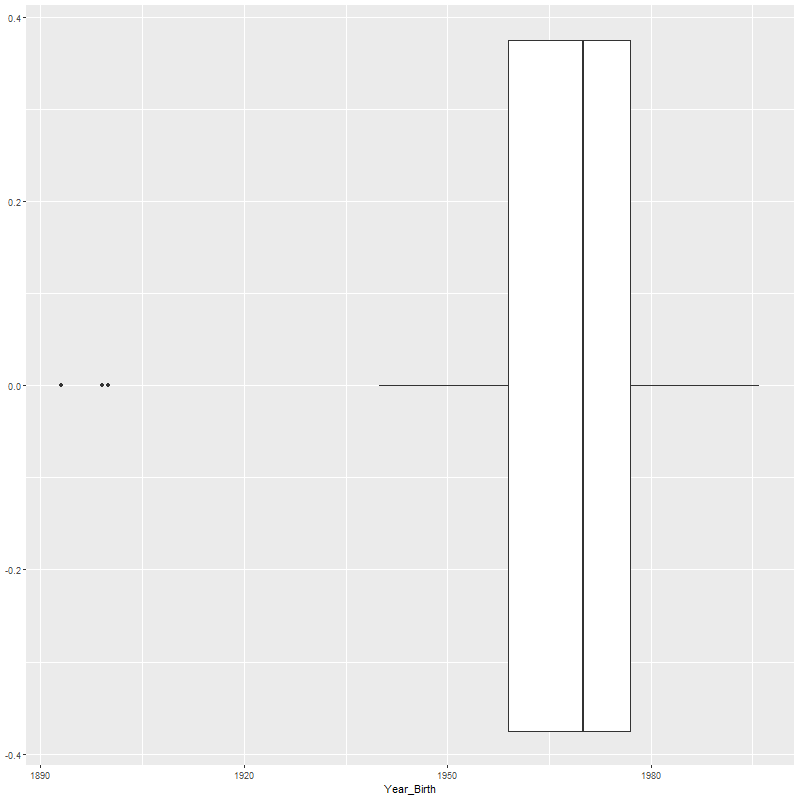
\includegraphics[width=0.4\textwidth]{Img/DESCRIPTION/DESCRIPTION001.png}
        }%
        \subfigure[BoxPlot Income]{%
            \label{fig:Histogram_Income}
            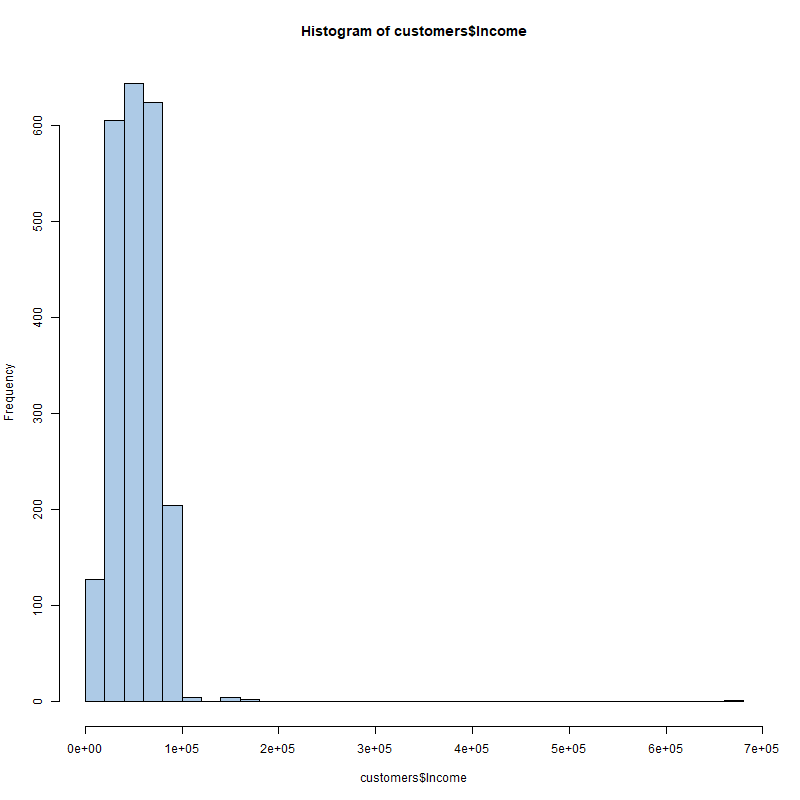
\includegraphics[width=0.4\textwidth]{Img/DESCRIPTION/DESCRIPTION020.png}
        }\\ %  ------- End of the first row ----------------------%
        \subfigure[BoxPlot KidHome]{%

            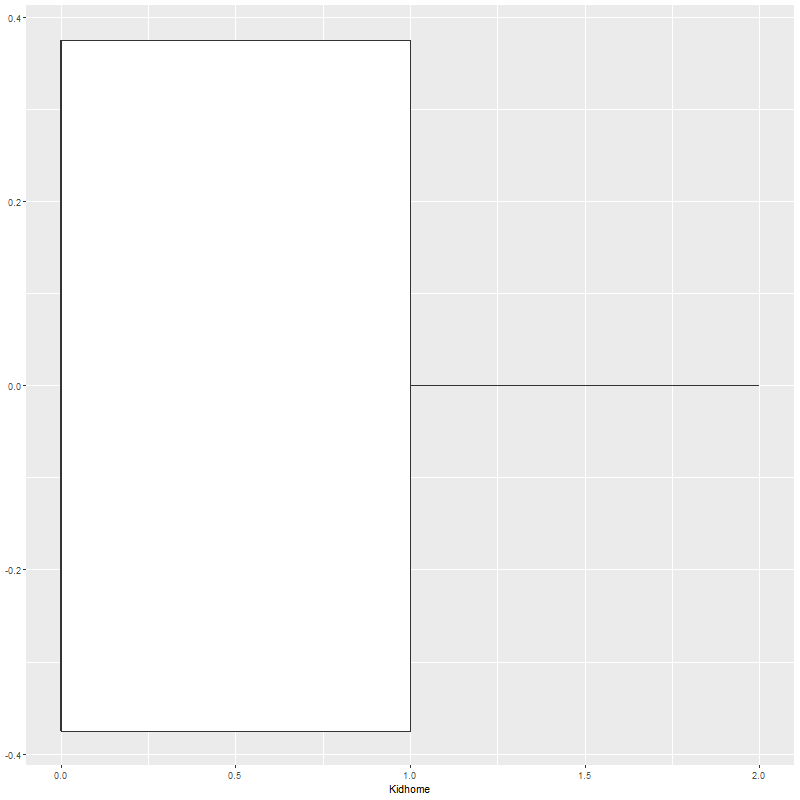
\includegraphics[width=0.4\textwidth]{Img/DESCRIPTION/DESCRIPTION004.png}
        }%
%
    \end{center}
\end{figure}
\begin{figure}[H]
     \begin{center}
%
        \subfigure[BoxPlot TeenHome]{%

            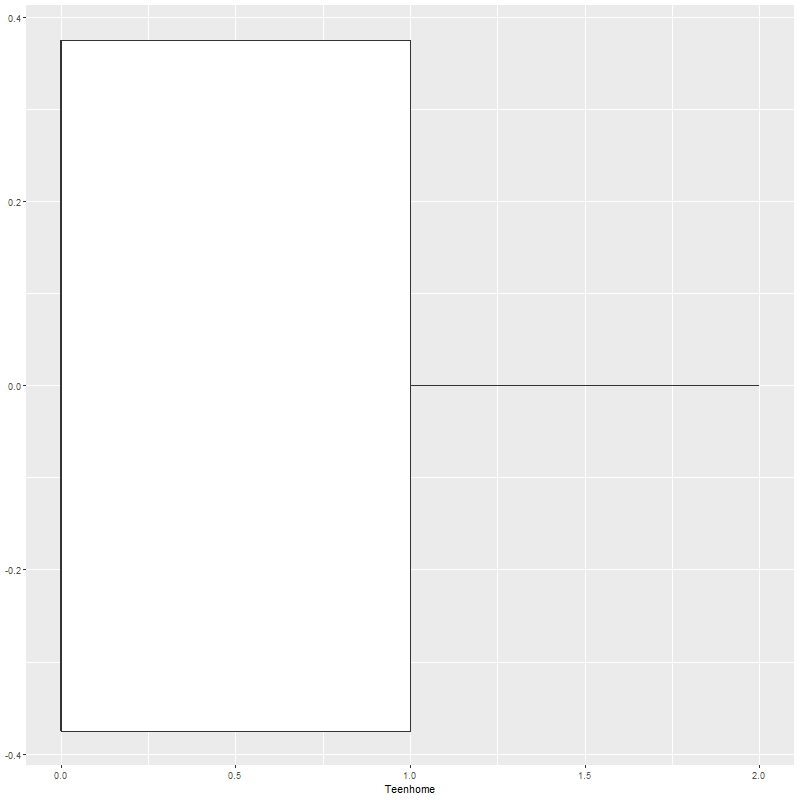
\includegraphics[width=0.4\textwidth]{Img/DESCRIPTION/DESCRIPTION005.png}
        }%
        \subfigure[BoxPlot Recency]{%

           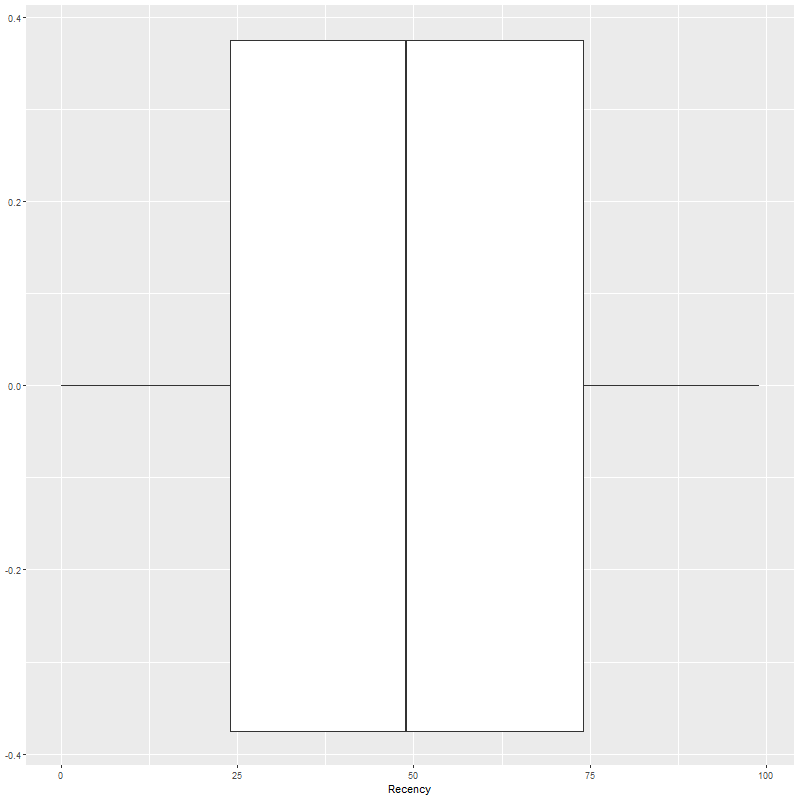
\includegraphics[width=0.4\textwidth]{Img/DESCRIPTION/DESCRIPTION006.png}
        }\\ %  ------- End of the first row ----------------------%
        \subfigure[BoxPlot MntWines]{%

            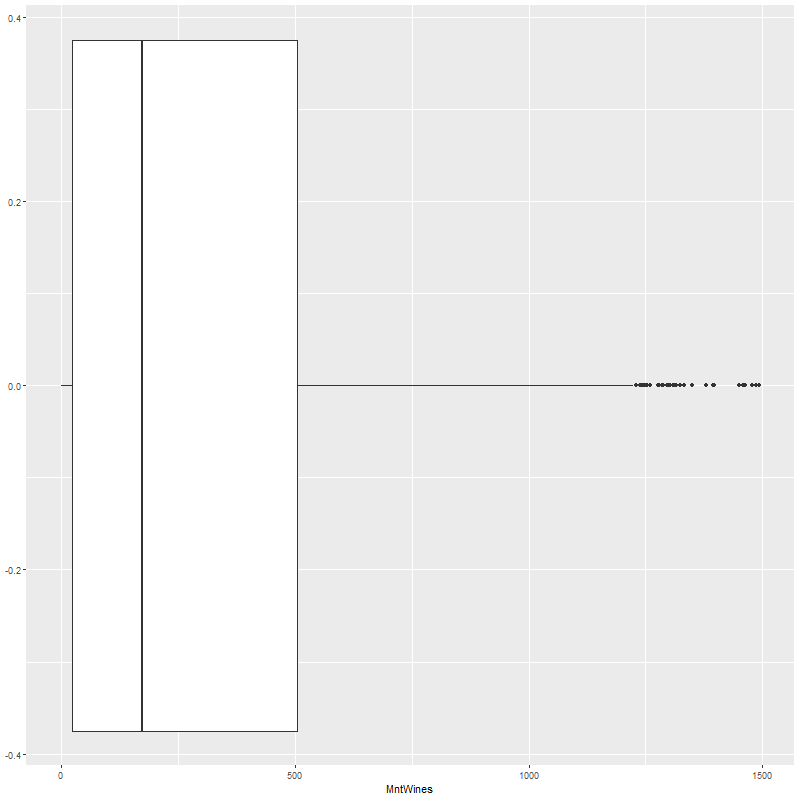
\includegraphics[width=0.4\textwidth]{Img/DESCRIPTION/DESCRIPTION007.png}
        }%
        \subfigure[BoxPlot MntFruits]{%

            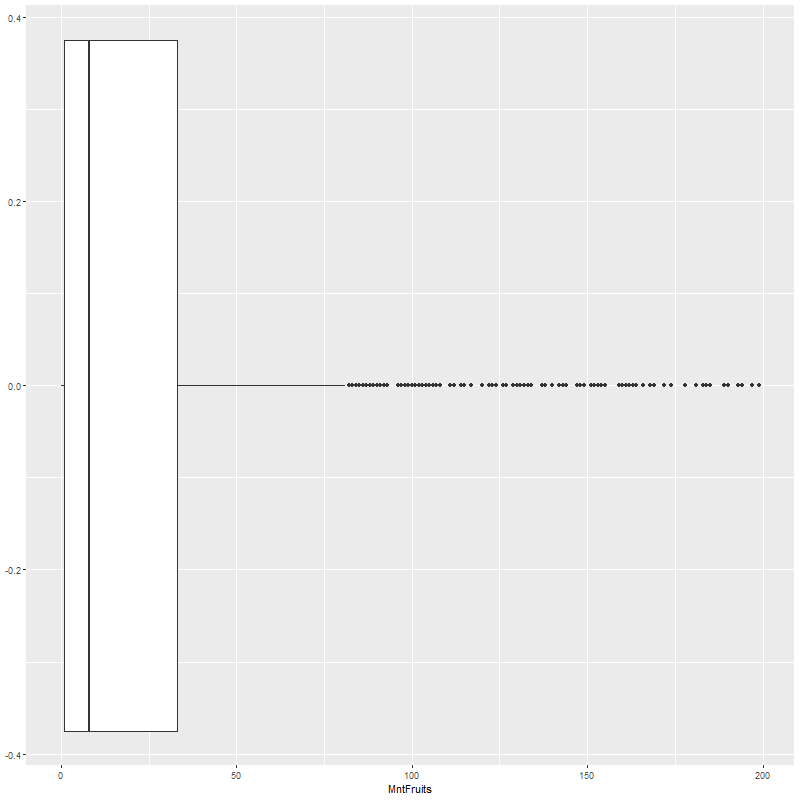
\includegraphics[width=0.4\textwidth]{Img/DESCRIPTION/DESCRIPTION008.png}
        }%
%
    \end{center}
\end{figure}
\begin{figure}[H]
     \begin{center}
%
        \subfigure[BoxPlot MntMeatProducts]{%

            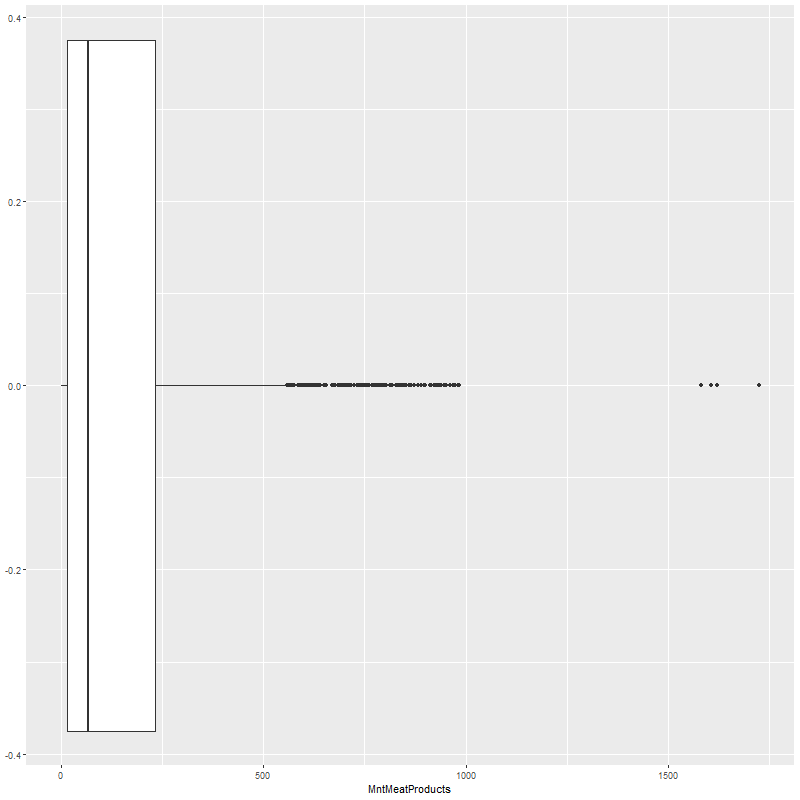
\includegraphics[width=0.4\textwidth]{Img/DESCRIPTION/DESCRIPTION009.png}
        }%
        \subfigure[BoxPlot MntFishProducts]{%

           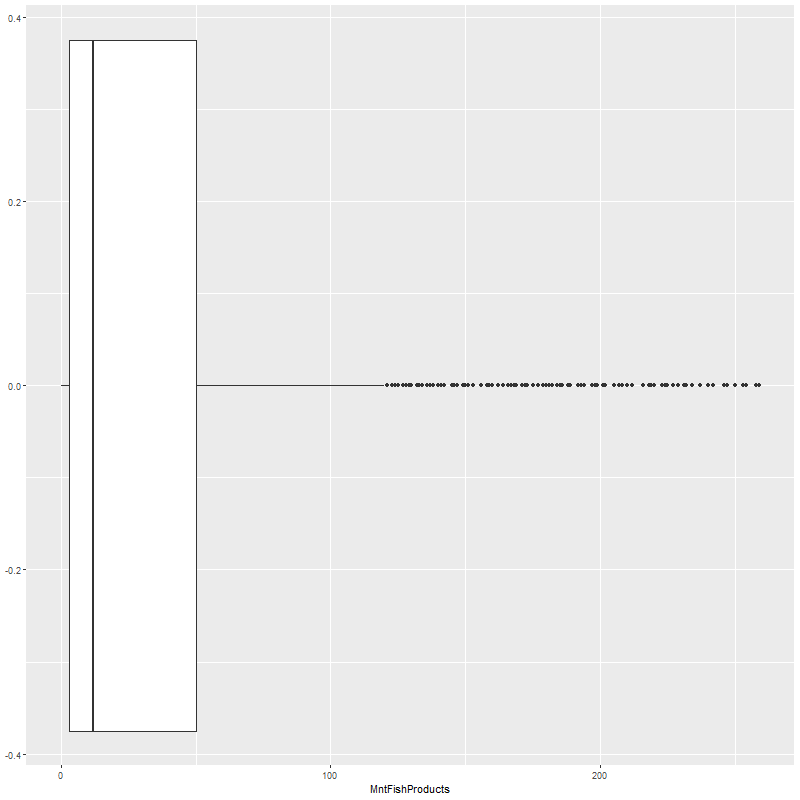
\includegraphics[width=0.4\textwidth]{Img/DESCRIPTION/DESCRIPTION010.png}
        }\\ %  ------- End of the first row ----------------------%
        \subfigure[BoxPlot MntSweetProducts]{%

            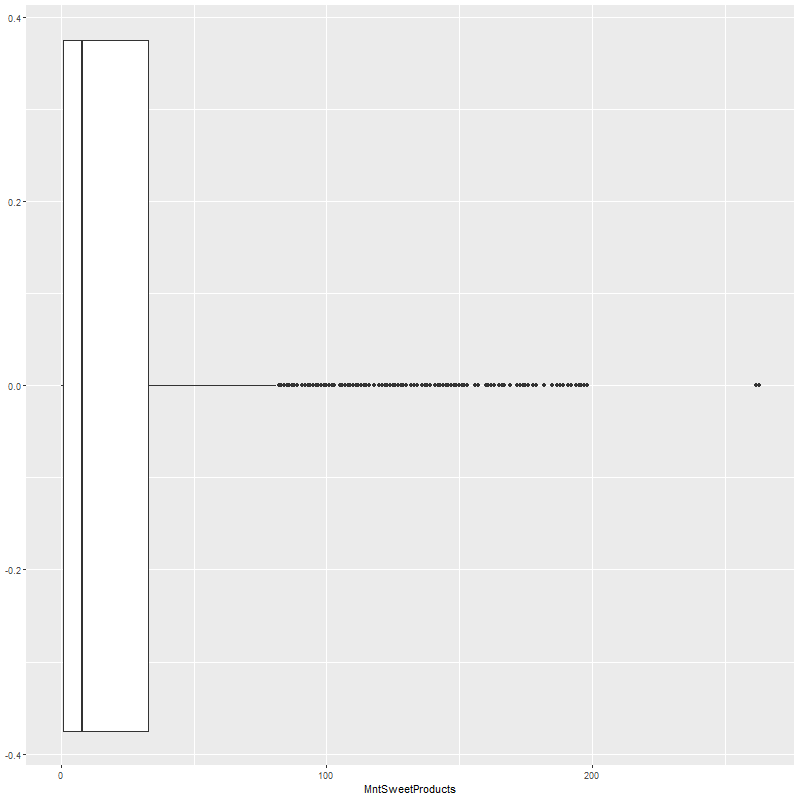
\includegraphics[width=0.4\textwidth]{Img/DESCRIPTION/DESCRIPTION011.png}
        }%
        \subfigure[BoxPlot MntGoldProds]{%

            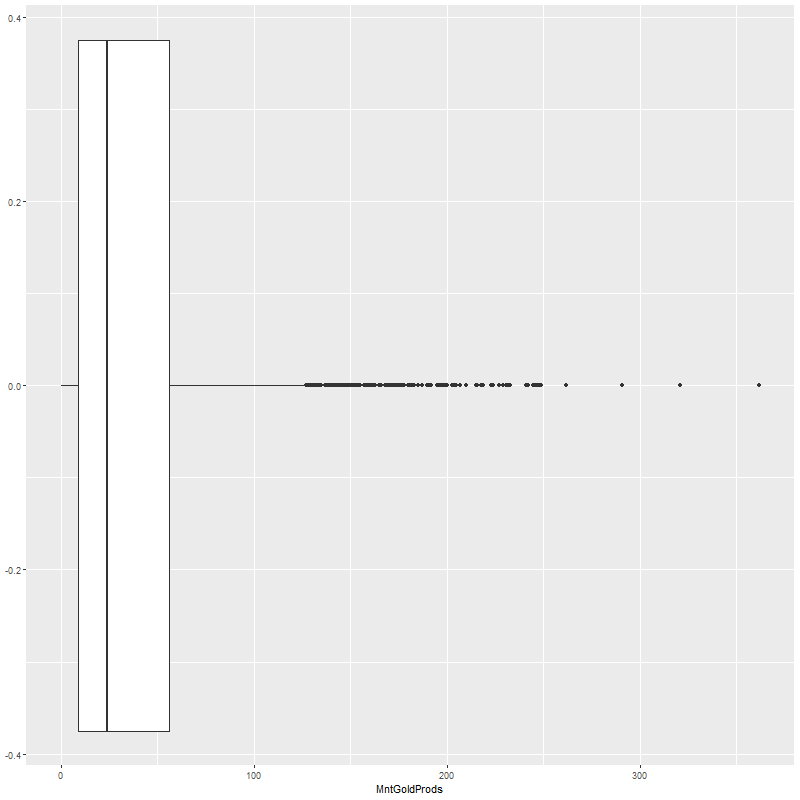
\includegraphics[width=0.4\textwidth]{Img/DESCRIPTION/DESCRIPTION012.png}
        }%
%
    \end{center}
\end{figure}
\begin{figure}[H]
     \begin{center}
%
        \subfigure[BoxPlot numDealsPurchases]{%

            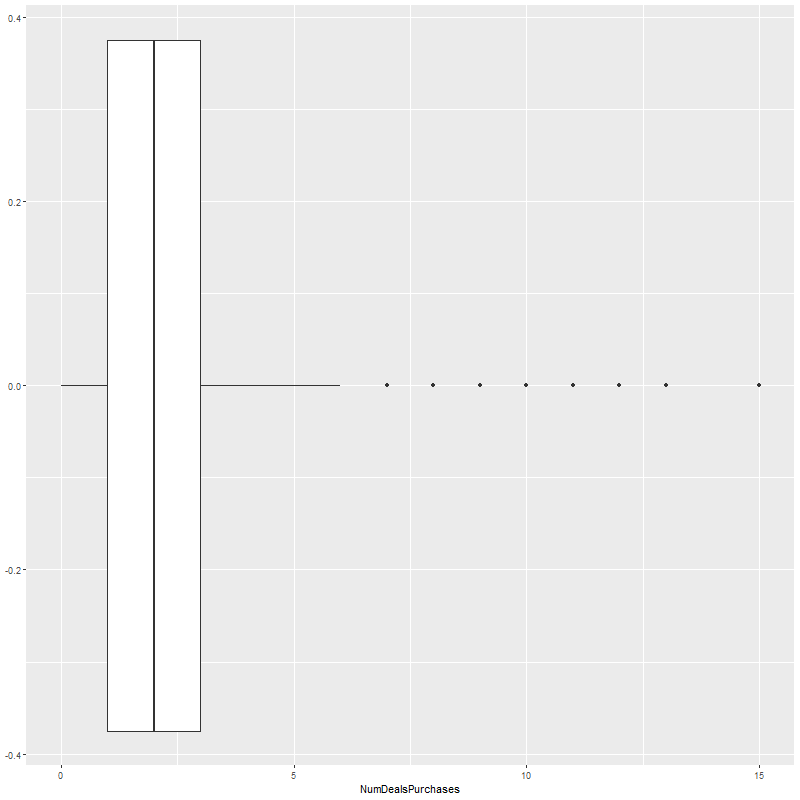
\includegraphics[width=0.4\textwidth]{Img/DESCRIPTION/DESCRIPTION013.png}
        }%
        \subfigure[BoxPlot NumWebPurchases]{%

           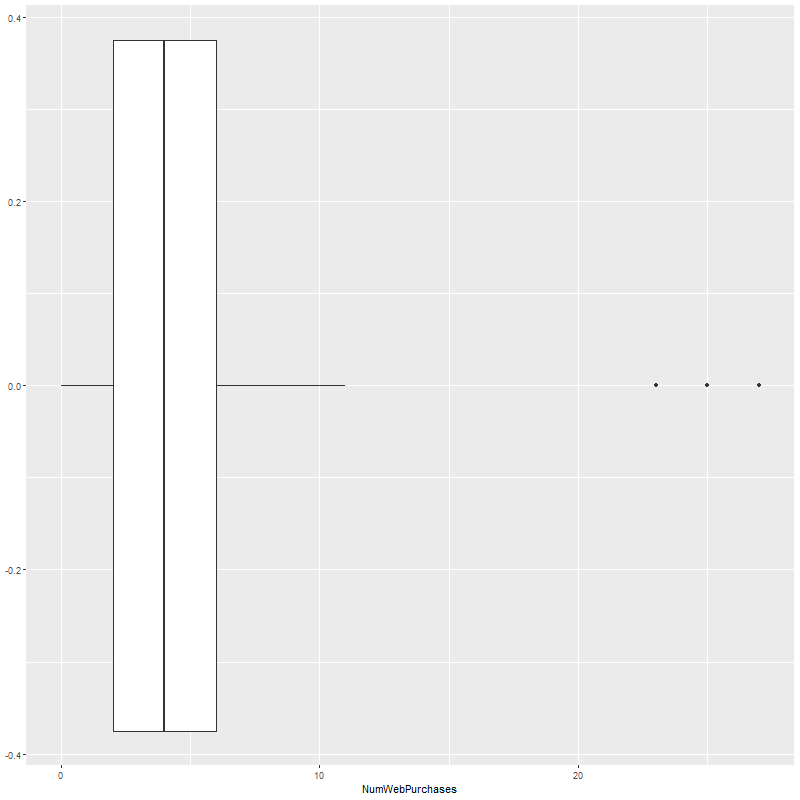
\includegraphics[width=0.4\textwidth]{Img/DESCRIPTION/DESCRIPTION014.png}
        }\\ %  ------- End of the first row ----------------------%
        \subfigure[BoxPlot NumCatalogPurchases]{%

            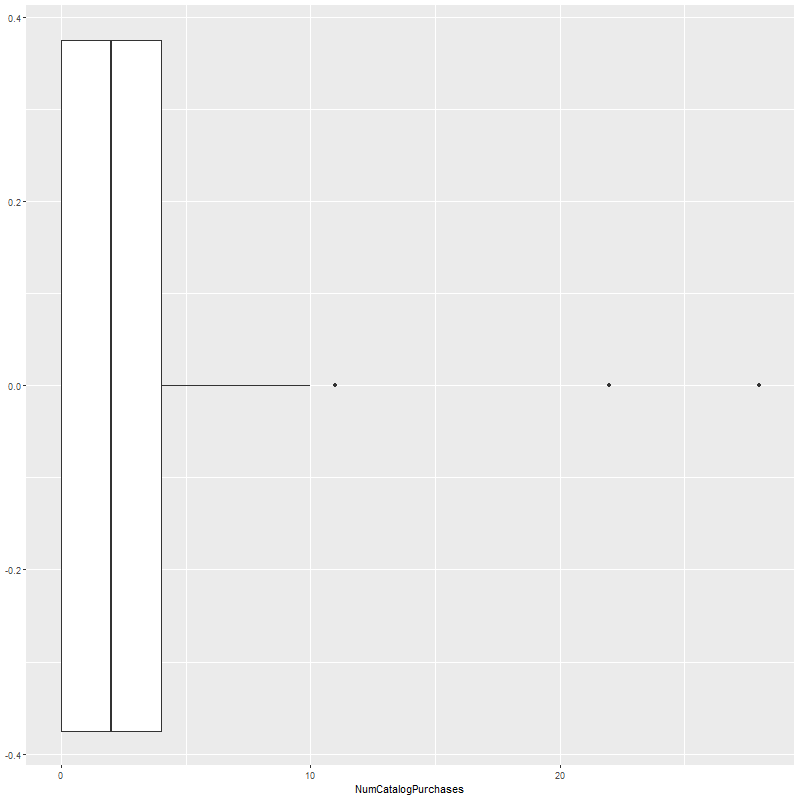
\includegraphics[width=0.4\textwidth]{Img/DESCRIPTION/DESCRIPTION015.png}
        }%
        \subfigure[BoxPlot NumStorePurchases]{%

            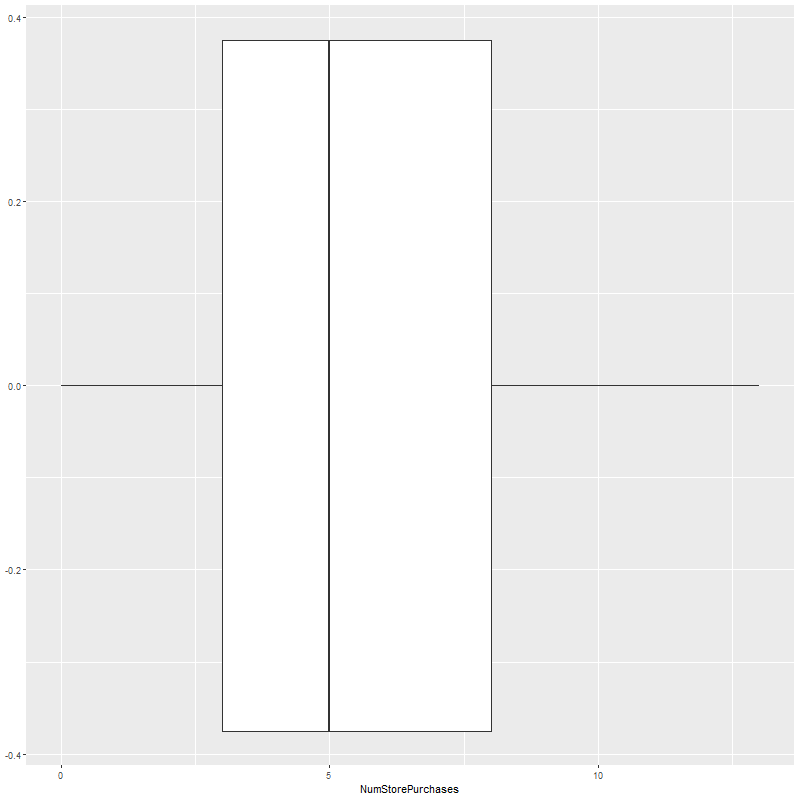
\includegraphics[width=0.4\textwidth]{Img/DESCRIPTION/DESCRIPTION016.png}
        }%
%
    \end{center}
\end{figure}
\begin{figure}[H]
     \begin{center}
%
        \subfigure[BoxPlot NumDealsPurchases]{%

            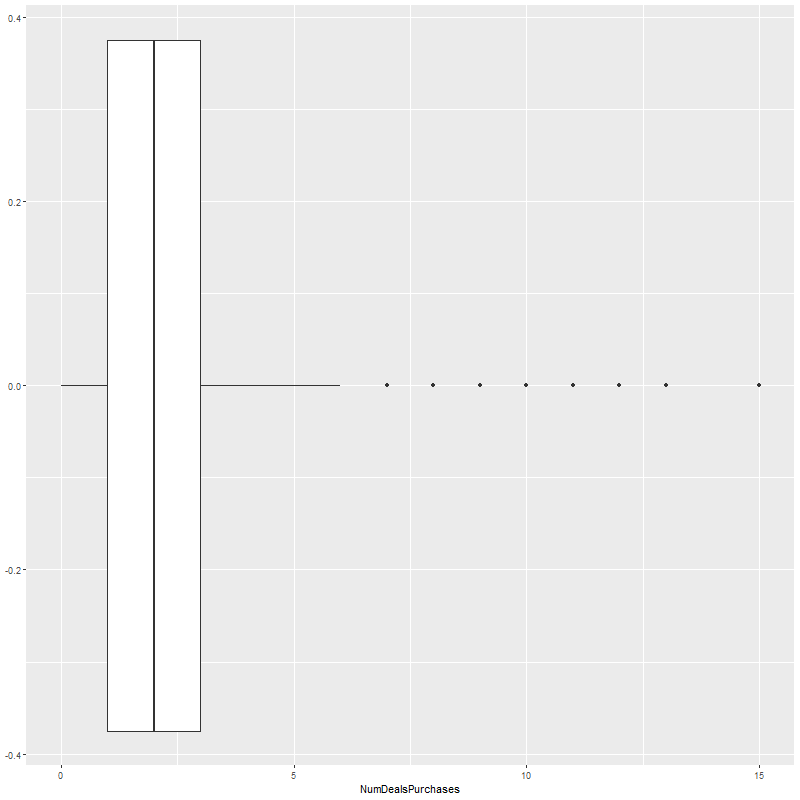
\includegraphics[width=0.4\textwidth]{Img/DESCRIPTION/DESCRIPTION017.png}
        }%
        \subfigure[BoxPlot Z\_CostContact]{%
            \label{fig:ZRevenue}
           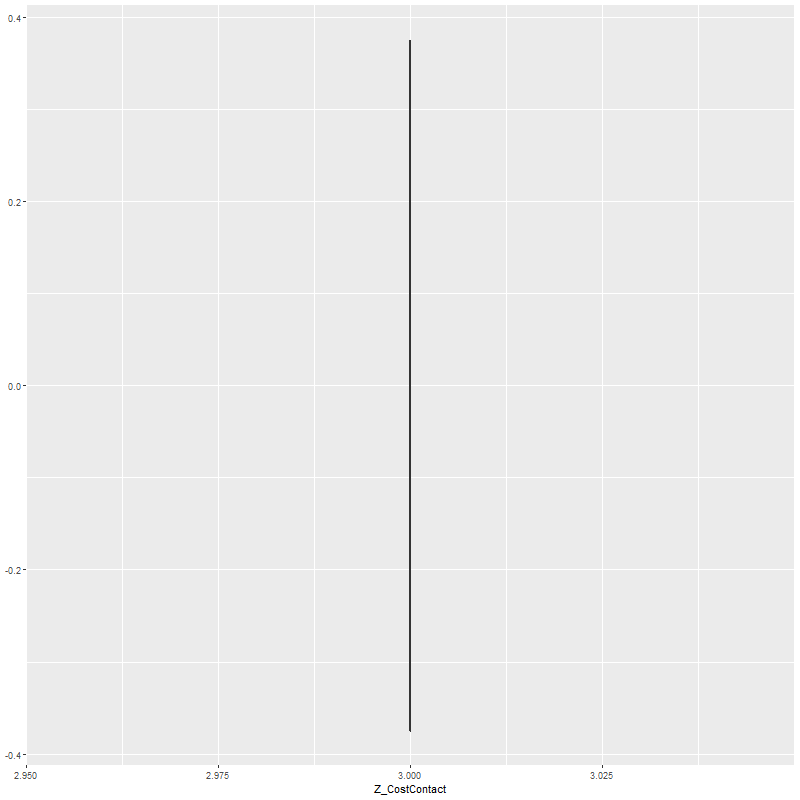
\includegraphics[width=0.4\textwidth]{Img/DESCRIPTION/DESCRIPTION018.png}
        }\\ %  ------- End of the first row ----------------------%
        \subfigure[BoxPlot Z\_Revenue]{%
            \label{fig:ZCostContact}
            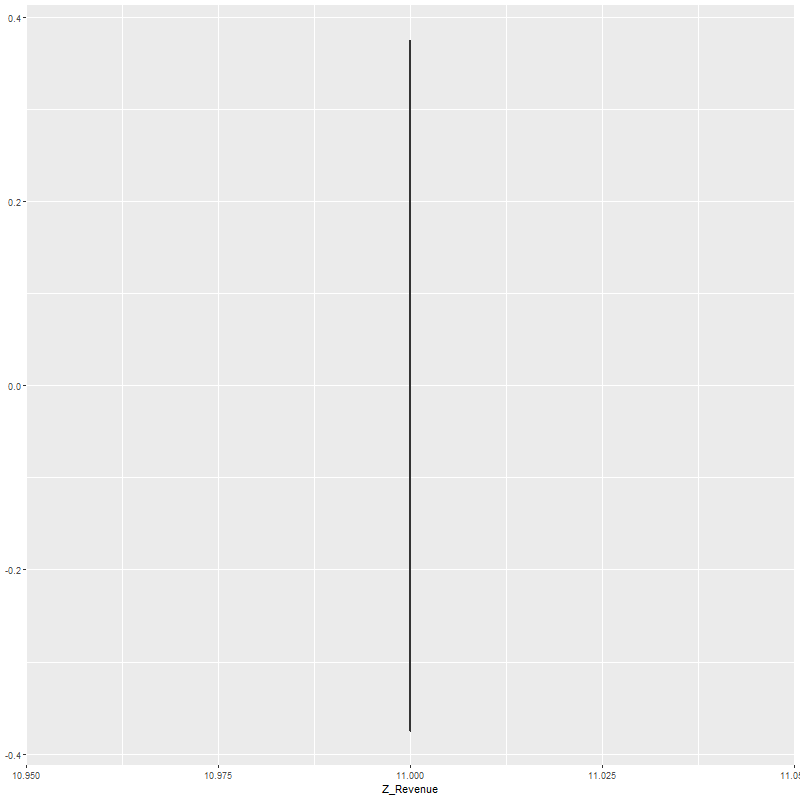
\includegraphics[width=0.4\textwidth]{Img/DESCRIPTION/DESCRIPTION019.png}
        }%
        \subfigure[BoxPlot Income]{%
            \label{fig:BoxPlotIncome}
            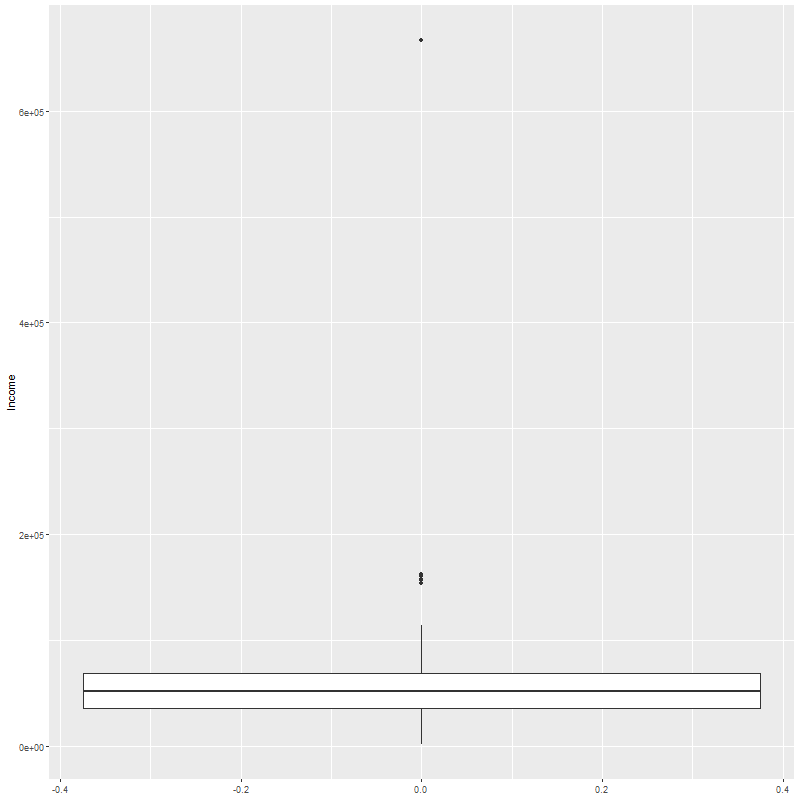
\includegraphics[width=0.4\textwidth]{Img/DESCRIPTION/DESCRIPTION021.png}
        }%
%
    \end{center}
\end{figure}

Durante questa prima indagine sono stati effettuati controlli di base sulle variabili. In particolare, dalle analisi dei boxplot riportati rispettivamente nelle figure \ref{fig:ZCostContact} e \ref{fig:ZRevenue} è doveroso notare la mancanza di \textbf{varianza} di tali variabili, questo aspetto sarà successivamente preso in considerazione durante la fase di preprocessing.\\ Inoltre durante l'analisi delle figure \ref{fig:BoxPlotIncome} e \ref{fig:Histogram_Income}, mediante un apposito \textit{warning} durante l'esecuzione del codice R, si è notata la presenza di alcuni valori mancanti.
\begin{lstlisting}[language=R]
hist(customers$Income,40,col="#adcae6")
ggplot(customers, aes(y = Income)) + geom_boxplot()
n_miss(customers) # counting the total number of missing values in the data
miss_var_summary(customers) # Summarizing missingness in each variable 
\end{lstlisting}
La tabella \ref{fig:miss_var_summary(customers)} mostra l'output del comando \textit{miss\_var\_summary(customers)}, dove si possono notare 24 valori mancanti nella variabile \textit{Income}.
\begin{table}[h!t]
\centering
\begin{tabular}{rlrr}
  \hline
 & variable & n\_miss & pct\_miss \\ 
  \hline
1 & Income &  24 & 1.07 \\ 
  2 & ID &   0 & 0.00 \\ 
  3 & Year\_Birth &   0 & 0.00 \\ 
  4 & Education &   0 & 0.00 \\ 
  5 & Marital\_Status &   0 & 0.00 \\ 
  6 & Kidhome &   0 & 0.00 \\ 
  7 & Teenhome &   0 & 0.00 \\ 
  8 & Dt\_Customer &   0 & 0.00 \\ 
  9 & Recency &   0 & 0.00 \\ 
  10 & MntWines &   0 & 0.00 \\ 
  11 & MntFruits &   0 & 0.00 \\ 
  12 & MntMeatProducts &   0 & 0.00 \\ 
  13 & MntFishProducts &   0 & 0.00 \\ 
  14 & MntSweetProducts &   0 & 0.00 \\ 
  15 & MntGoldProds &   0 & 0.00 \\ 
  16 & NumDealsPurchases &   0 & 0.00 \\ 
  17 & NumWebPurchases &   0 & 0.00 \\ 
  18 & NumCatalogPurchases &   0 & 0.00 \\ 
  19 & NumStorePurchases &   0 & 0.00 \\ 
  20 & NumWebVisitsMonth &   0 & 0.00 \\ 
  21 & AcceptedCmp3 &   0 & 0.00 \\ 
  22 & AcceptedCmp4 &   0 & 0.00 \\ 
  23 & AcceptedCmp5 &   0 & 0.00 \\ 
  24 & AcceptedCmp1 &   0 & 0.00 \\ 
  25 & AcceptedCmp2 &   0 & 0.00 \\ 
  26 & Complain &   0 & 0.00 \\ 
  27 & Z\_CostContact &   0 & 0.00 \\ 
  28 & Z\_Revenue &   0 & 0.00 \\ 
  29 & Response &   0 & 0.00 \\ 
   \hline
\end{tabular}

    \caption{Output funzione \textit{miss\_var\_summary(customers)}}
   
   \label{fig:miss_var_summary(customers)}
\end{table}
\subsection{Data Preprocessing}
La fase di \textit{data preprocessing} è risultata fondamentale per la buona riuscita dell'analisi dei dati preposti. Essa si basa su quattro principali stadi:
\begin{itemize}
    \item Refactor del dataset
    \item Risoluzione dei valori mancanti nella variabile \textit{income}
    \item Splitting del dataset in \textit{trainingSet} e \textit{testSet}
    \item Feature Scaling
\end{itemize}
\subsubsection{Refactor del Dataset}
In questa fase ci si è concentrati su diversi aspetti migliorativi. In primo luogo si è voluto essettuare un'azione di incorporamento di dati. La motivazione è dovuta principalmente alla presenza di dati ridondati all'interno di molte variabili, in particolare si vuole porre l'attenzione su: \textit{Marital\_Status} e \textit{Education}. Difatti utilizzando la funzione \textit{unique}, come riportato nelle tabelle \ref{fig:unique(customersEducation)} e \ref{fig:unique(customersMaritalStatus)}, si è potuto rilevare la presenza di troppi elementi superflui.
\begin{table}[h!t]
\centering
\begin{tabular}{rl}
  \hline
 & unique(customers\$Marital\_Status) \\ 
  \hline
1 & Single \\ 
  2 & Together \\ 
  3 & Married \\ 
  4 & Divorced \\ 
  5 & Widow \\ 
  6 & Alone \\ 
  7 & Absurd \\ 
  8 & YOLO \\ 
  \hline
\end{tabular}
\caption{Output $unique(customers\$Marital\_Status)$}
\label{fig:unique(customersMaritalStatus)}
\end{table}

\begin{table}[h!t]
\centering
\begin{tabular}{rl}
  \hline
 & unique(customers\$Education) \\ 
  \hline
1 & Graduation \\ 
  2 & PhD \\ 
  3 & Master \\ 
  4 & Basic \\ 
  5 & 2n Cycle \\ 
  \hline
\end{tabular}
\caption{Output $unique(customers\$Education)$}
\label{fig:unique(customersEducation)}
\end{table}

Come mostrato dal codice sottostante, l'obiettivo è stato quello di diminuire, per favorire l'analisi mediante i diversi algoritmi utilizzati, in numero delle categorie di valori per le relative variabili. 
\begin{lstlisting}[language=R]
# ------------------------------------- COLLAPSING
#Collapsing marital Status into two categories: Single & Couple
unique(customers$Marital_Status)
customers <- mutate(customers, Marital_Status = replace(Marital_Status, Marital_Status == "Divorced" | Marital_Status == "Widow" | Marital_Status == "Alone" | Marital_Status == "Absurd" | Marital_Status == "YOLO", "Single"))
customers <- mutate(customers, Marital_Status = replace(Marital_Status, Marital_Status == "Together" | Marital_Status == "Married", "Couple"))

#Collapsing the Education into two Categories: graduate and non-graduate
unique(customers$Education)
customers <- mutate(customers, Education = replace(Education, Education == "Graduation"| Education == "PhD" | Education == "Master", "graduate"))
customers <- mutate(customers, Education = replace(Education, Education == "Basic"| Education == "2n Cycle", "non-graduate"))
# ------------------------------------- 
\end{lstlisting}
In particolar modo si è deciso di fornire due possibili valori riassuntivi per ciascuna variabile, come indicato nelle tabelle \ref{fig:unique(customersEducation)2} e \ref{fig:unique(customersMaritalStatus)2}.

\begin{table}[h!t]
\centering
\begin{tabular}{rl}
  \hline
 & unique(customers\$Education) \\ 
  \hline
1 & graduate \\ 
  2 & non-graduate \\ 
   \hline
\end{tabular}
\caption{Output $unique(customers\$Education)$ dopo la procedura di \textit{collapsing} dei dati}
\label{fig:unique(customersEducation)2}
\end{table}


\begin{table}[h!t]
\centering
\begin{tabular}{rl}
  \hline
 & unique(customers\$Marital\_Status) \\ 
  \hline
1 & Single \\ 
  2 & Couple \\ 
   \hline
\end{tabular}
\caption{Output $unique(customers\$Marital\_Status)$ dopo la procedura di \textit{collapsing} dei dati}
\label{fig:unique(customersMaritalStatus)2}
\end{table}

La fase di \textit{refactoring} si è anche occupata della convesione in \textit{factor} degli elementi \textit{character} all'interno dell'insieme di dati.
Il codice sottostante mostra la procedura seguita. Le tabelle \ref{fig:head(customersEducation)} e \ref{fig:head(customersMaritalStatus)} mostrano il risultato di tale procedura.
\begin{lstlisting}[language=R]
# ------------------------------------- CONVERSION
#Converting them to factors
customers <- mutate(customers, Marital_Status = as.factor(Marital_Status), Education = as.factor(Education))

# Encoding the categorical features to numeric
customers <- mutate(customers, Education = case_when(Education == "graduate" ~ 1,
                                                     Education == "non-graduate" ~ 0))
customers <- mutate(customers, Marital_Status = case_when(Marital_Status == "Couple" ~ 1,
                                                          Marital_Status == "Single" ~ 0))
# ------------------------------------- 
\end{lstlisting}

\begin{table}[h!t]
\centering
\begin{tabular}{rr}
  \hline
 & head(customers\$Marital\_Status) \\ 
  \hline
1 & 0.00 \\ 
  2 & 0.00 \\ 
  3 & 1.00 \\ 
  4 & 1.00 \\ 
  5 & 1.00 \\ 
  6 & 1.00 \\ 
   \hline
\end{tabular}
\caption{Output $head(customers\$Marital\_Status)$}
\label{fig:head(customersMaritalStatus)}
\end{table}
\begin{table}[h!t]
\centering
\begin{tabular}{rr}
  \hline
 & head(customers\$Education) \\ 
  \hline
1 & 1.00 \\ 
  2 & 1.00 \\ 
  3 & 1.00 \\ 
  4 & 1.00 \\ 
  5 & 1.00 \\ 
  6 & 1.00 \\ 
   \hline
\end{tabular}
\caption{Output $head(customers\$Education)$}
\label{fig:head(customersEducation)}
\end{table}

Questa fase si è anche occupata della creazione di nuove variabili partendo da quelle già presenti all'interno da quelle già esistenti. Si ponga l'attenzione in particolar modo alle \textbf{categorie} di variabili \textit{Mnt}, \textit{Accepted}, \textit{KidHome}, \textit{TeenHome}. Tali categorie possono essere sommate per creare nuove variabili riassuntive. Il codice seguente e la tabella \ref{fig:Totalspent&TotalCampains&TotalChilds} ne riportano un esempio:
\begin{lstlisting}[language=R]
# ------------------------------------- TOTAL
#Creating a new variable:Total_spent
customers <- mutate(customers, Total_spent = MntWines + MntFruits + MntMeatProducts + MntFishProducts + MntSweetProducts + MntGoldProds)

# Details about previous campains also combined. Creating a new variable:Total_Campains
customers <- mutate(customers, Total_Campains = AcceptedCmp1 + AcceptedCmp2 + AcceptedCmp3 + AcceptedCmp4 + AcceptedCmp5)

# These variables can be combined and we can get the no of children for the customers. Creating a new variable:Total_Childs
customers <- mutate(customers, Total_Childs = Kidhome + Teenhome)
# ------------------------------------- 
\end{lstlisting}
\begin{table}[h!t]
\centering
\begin{tabular}{rrrr}
  \hline
 & Total\_spent & Total\_Campains & Total\_Childs \\ 
  \hline
1 & 1617 &   0 &   0 \\ 
  2 &  27 &   0 &   2 \\ 
  3 & 776 &   0 &   0 \\ 
  4 &  53 &   0 &   1 \\ 
  5 & 422 &   0 &   1 \\ 
  6 & 716 &   0 &   1 \\ 
   \hline
\end{tabular}
\caption{Primi valori delle variabili Total\_spent \& Total\_Campains \& Total\_Childs}
\label{fig:Totalspent&TotalCampains&TotalChilds}
\end{table}

Per finire è doveroso sottolineare che in questa sezioni ci si è anche occupati dell'eliminazione delle variabili superflue, come \textit{Z\_CostContact} e \textit{Z\_Revenue} che non hanno varianza, e della sostituzione della varibile \textit{Year\_Birth} con \textit{Age}.
\begin{lstlisting}[language=R]
# we can calculate customer age from the birth year. It will be more usefull to our analysis.
# creating a new variable Age from Year of Birth 
thisYear <- as.numeric(format(as.Date(Sys.Date(), format="%d-%m-%Y"),"%Y"))
thisYear
customers <- mutate(customers, Age = thisYear - Year_Birth)


#Dropping some redundant features
customers <- select(customers, - ID, - Year_Birth, - Z_CostContact, - Z_Revenue, -Dt_Customer)
\end{lstlisting}
\subsubsection{Risoluzione dei valori mancanti}
Come mostrato nel codice sottostante, non si è deciso di eliminare completamente i valori mancanti all'interno della variabile \textit{income}, bensì si è adottata un'altra strategia: la sostituzione con il valore medio della variabile stessa.
\begin{lstlisting}[language=R]
customers$Income <- ifelse(is.na(customers$Income), # is.na check is a value is not available
                          ave(customers$Income, FUN = function(x) mean(x, na.rm = TRUE)), # if is not available change with average
                          customers$Income # else
) 
\end{lstlisting}
\subsubsection{Splitting in TrainingSet e TestSet}
Al fine di una buona analisi dei dati, si è deciso di suddividere il dataset iniziale in due più ridotti: l'insieme di allenamento e quello di testing. Il codice sottostante mostra la procedura effettuata.
\begin{lstlisting}[language=R]
set.seed(17538)
split <- sample.split(customers$Response, SplitRatio = 0.8)
trainingSet <- subset(customers, split == TRUE)
testSet <- subset(customers, split == FALSE)
\end{lstlisting}
\subsubsection{Feature Scaling}
E' opportuno sottolineare che si è deciso di normalizzare i valori delle variabili al fine di poter utilizzare al meglio gli algoritmi di machine learning che verranno descritti nel corso di questa trattazione. Il codice seguente mostra un esempio:
\begin{lstlisting}[language=R]
trainingSet_scaled <- as.data.frame(scale(trainingSet[, getIndipendentNumbersOfCol()]))
testSet_scaled <- as.data.frame(scale(testSet[, getIndipendentNumbersOfCol()]))
\end{lstlisting}


\subsection{EDA}
Dopo aver eseguito il preprocessing dei dati si è passati ad un'analisi esplorativa dei dati mutando i valori che può assumere una certa variabile tramite la funzione \textit{cut}. 
Questa operazione è stata eseguita per \textit{Age}, \textit{Income} e Total spent. 

\begin{lstlisting}[language=R]
# Age Range
ageRange <- cut(trainingSet$Age, breaks = c(24, 64, Inf), include.lowest = T,
                ordered_result = T, labels = c("Adult", "Senior"))
trainingSet <- mutate(trainingSet, Age_range = ageRange)

# Income Range
incomeRange <- cut(trainingSet$Income, 
                   calculateBreaksFromSummary(trainingSet$Income),
                   labels = c("low", "low medium", "medium high", "high"))
trainingSet <- mutate(trainingSet, Income_range = incomeRange)

# Spent Range
spentRange <- cut(trainingSet$Total_spent, 
                  calculateBreaksFromSummary(trainingSet$Total_spent),
                  labels = c("low", "low medium", "medium high", "high"))
trainingSet <- mutate(trainingSet, Spent_range = spentRange)
\end{lstlisting}

\begin{figure}[H]
     \begin{center}
%
        \subfigure[PiePlot Year\_Birth]{%

            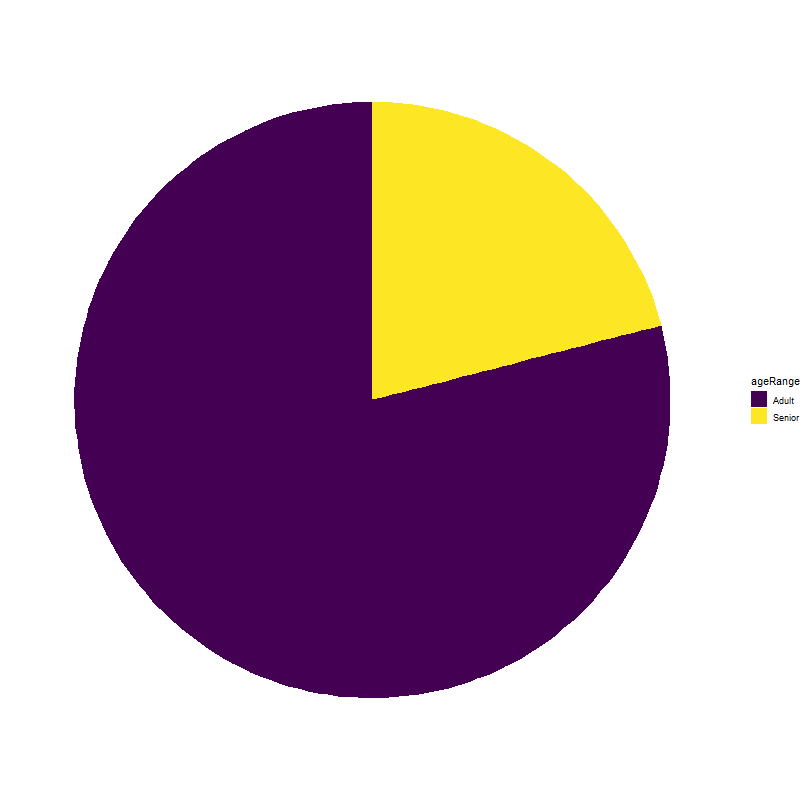
\includegraphics[width=0.45\textwidth]{Img/EDA/EDA001.png}
        }%
        \subfigure[PiePlot Income]{%
            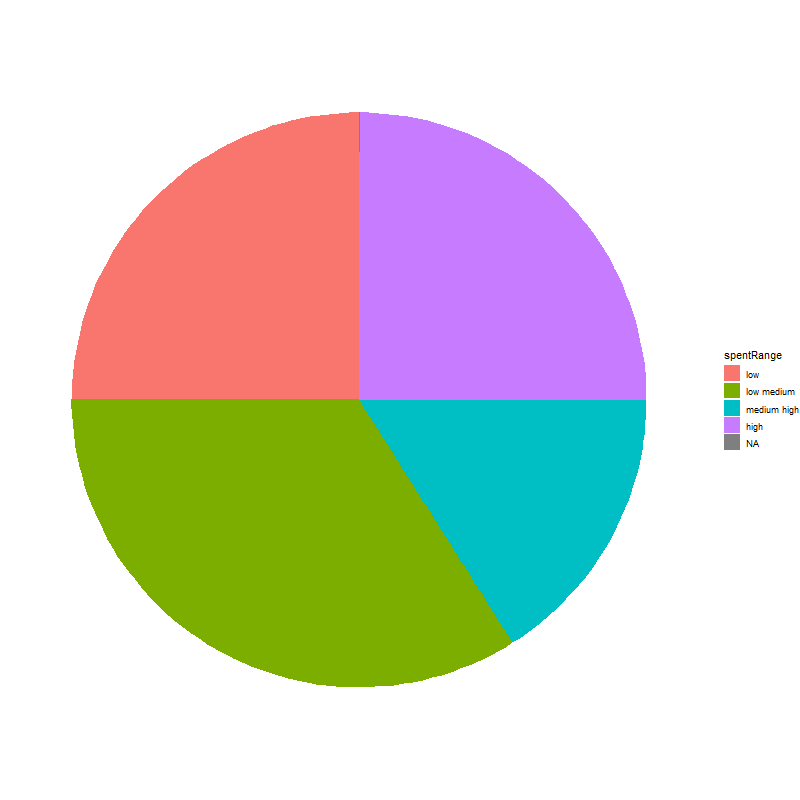
\includegraphics[width=0.5\textwidth]{Img/EDA/EDA004.png}
        }\\ %  ------- End of the first row ----------------------%
        \subfigure[PiePlot di Marital\_Status]{%

            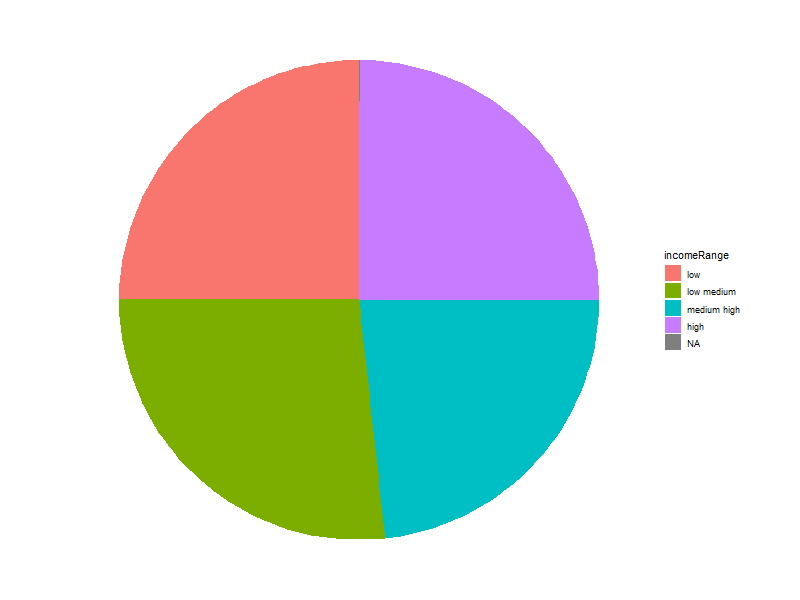
\includegraphics[width=0.5\textwidth]{Img/EDA/EDA005.png}
        }%
%
    \end{center}
\end{figure}


Il primo grafico a torta (t) è relativo alla variabile Age, il colore viola rappresenta il valore \textit{Adult} mentre il colore giallo \textit{Senior}. Dal grafico si ricava che la maggior parte degli individui è \textit{Adult}.
Il secondo rappresenta la variabile \textit{income}, il dataset è equi-distribuito in questo caso.
La distribuizione dei valori che assume la variabile \textit{Total spent} è raffigurata nella Figura 3. Da essa si ricava che low e high sono simili mentre quello più frequente è \textit{low medium}.\\
Inoltre si può notare facendo l'istogramma della variabile \textit{Age}che l'età media degli individui presenti nel dataset è superiore ai 50 anni e la maggioranza ha un titolo di studio maggiore o uguale alla laurea.


\begin{figure}[H]
     \begin{center}
%
        \subfigure[Istogramma di Age.]{%

            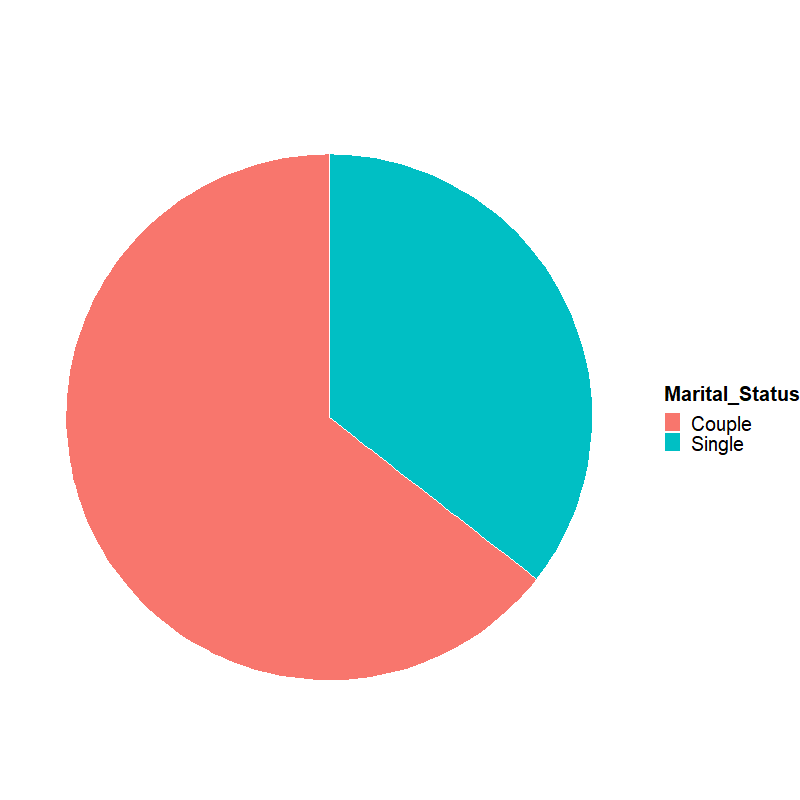
\includegraphics[width=0.4\textwidth]{Img/EDA/EDA002.png}
            \label{fig:IstogrammaAge}
        }%
        \subfigure[Istogramma di Income.]{%
            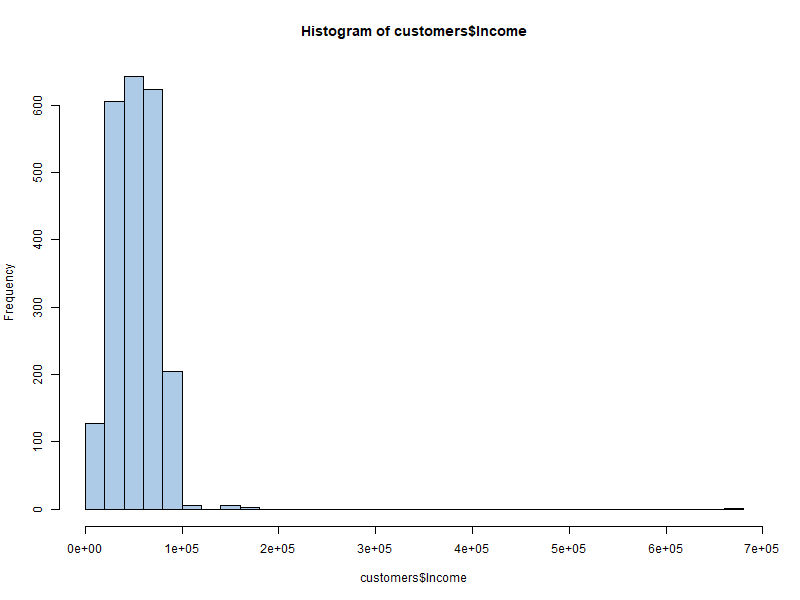
\includegraphics[width=0.4\textwidth]{Img/EDA/EDA007.png}
            \label{fig:IstogrammaIncome}
        }\\ %  ------- End of the first row ----------------------%
%
\subfigure[Istogramma di Education.]{%
            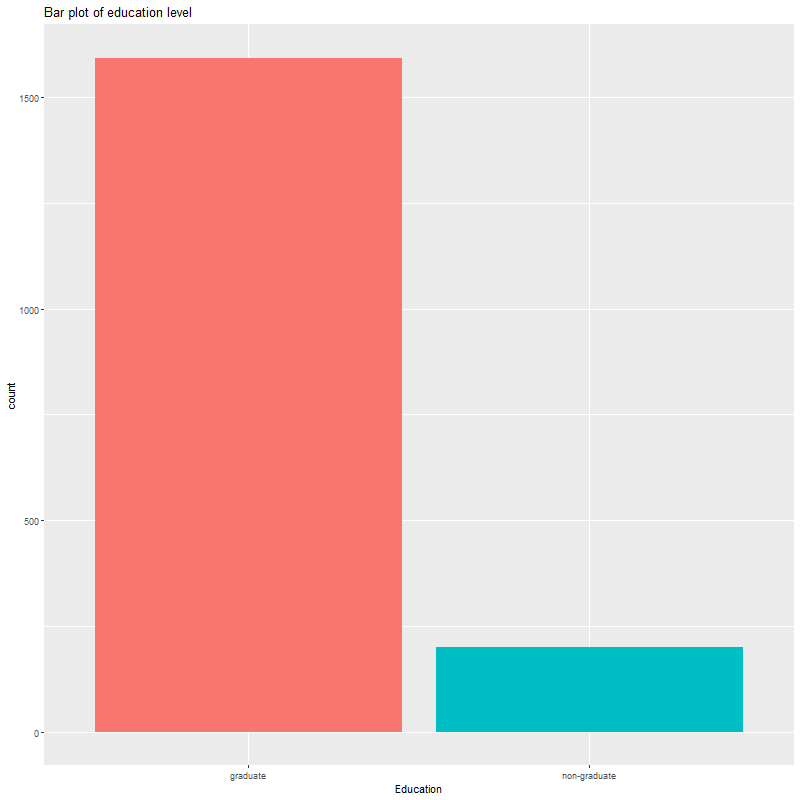
\includegraphics[width=0.4\textwidth]{Img/EDA/EDA003.png}
            \label{fig:IstogrammaEducation}
        }\\ %  ------- End of the first row ----------------------%
%
\subfigure[BoxPlot di Education.]{%
            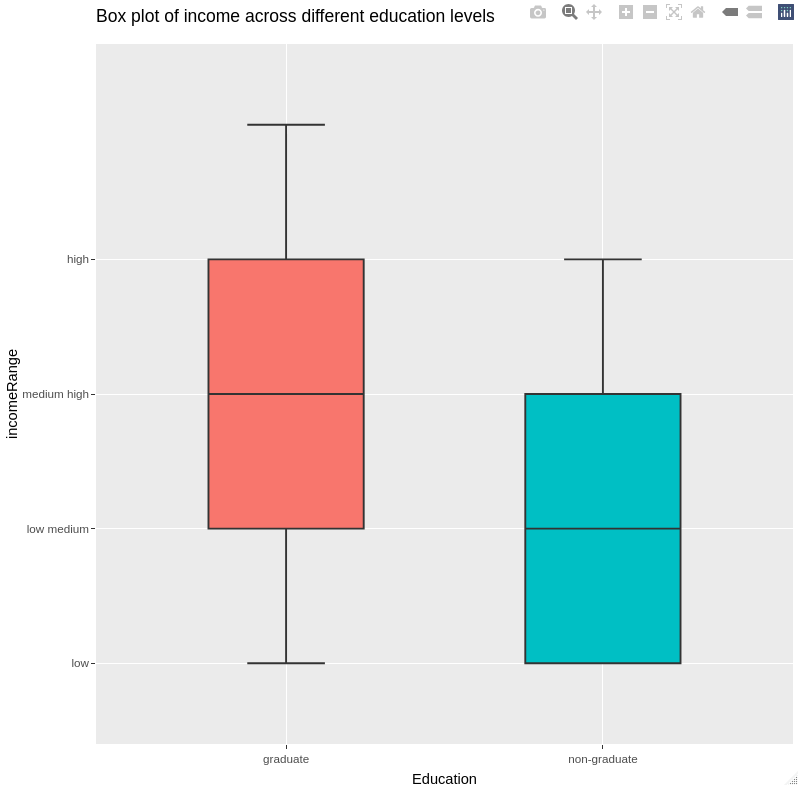
\includegraphics[width=0.4\textwidth]{Img/EDA/EDA054.png}
            \label{fig:BoxPlotEducation}
        }\\ %  ------- End of the first row ----------------------%
%

    \end{center}
\end{figure}

\newpage
\subsubsection{Total Children}
La maggior parte delle istanze del dataset ha 1 figlio, la variabile Total\_Children è la somma tra la variabile KidHome e TeenHome. Questa informazione si è ricavata eseguendo il codice riportato i seguito.\\

\begin{lstlisting}[language=R]
ggplot(trainingSet, aes(x=Total_Childs)) + geom_histogram(binwidth = 0.5, colour = "Black")
\end{lstlisting}

\begin{figure}[h]
    \centering
    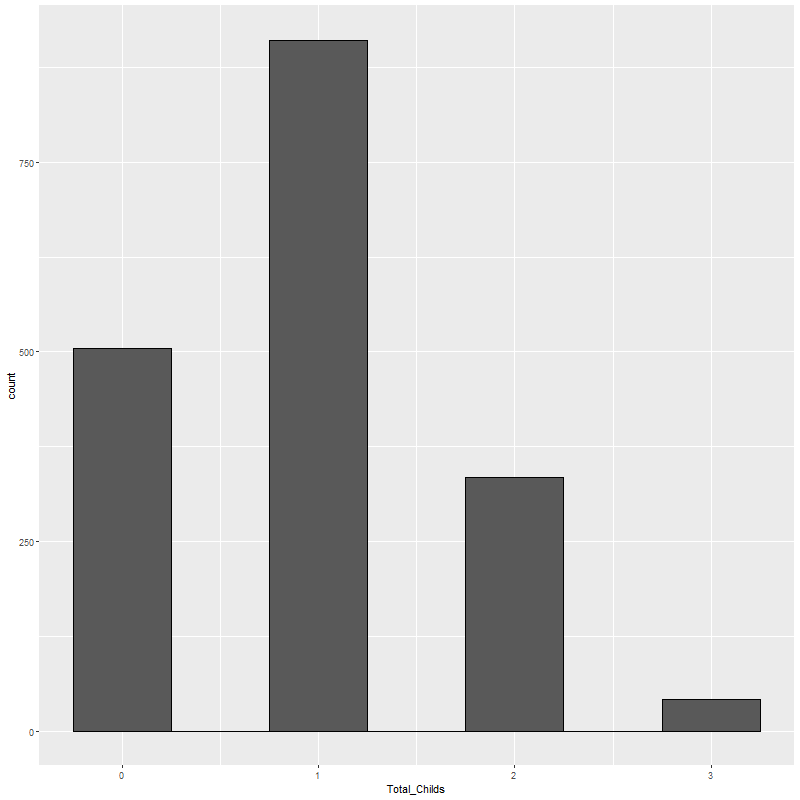
\includegraphics[width=.4\textwidth]{Img/EDA/EDA015.png}
    \caption{hist plot di total\_children }
    \label{fig:IstogrammaTc}
\end{figure}

\paragraph{Total\_Childen e Age}
Si è analizzata anche la relazione tra il numero totale di figli, \textit{Total\_children} ed \textit{Age} ed è risultato che tra gli \textit{Adult} il numero di figli più frequente è 1 e che rispetto ai \textit{Senior} hanno più figli.

\begin{lstlisting}[language=R]
age_children_histogram <- ggplot(trainingSet, aes(x=Total_Spent)) + geom_histogram(aes(fill=Age_range), binwidth = 0.5, colour = "Black")
age_children_histogram + facet_grid(Age_range~.)
\end{lstlisting}
\begin{figure}[h]
    \centering
    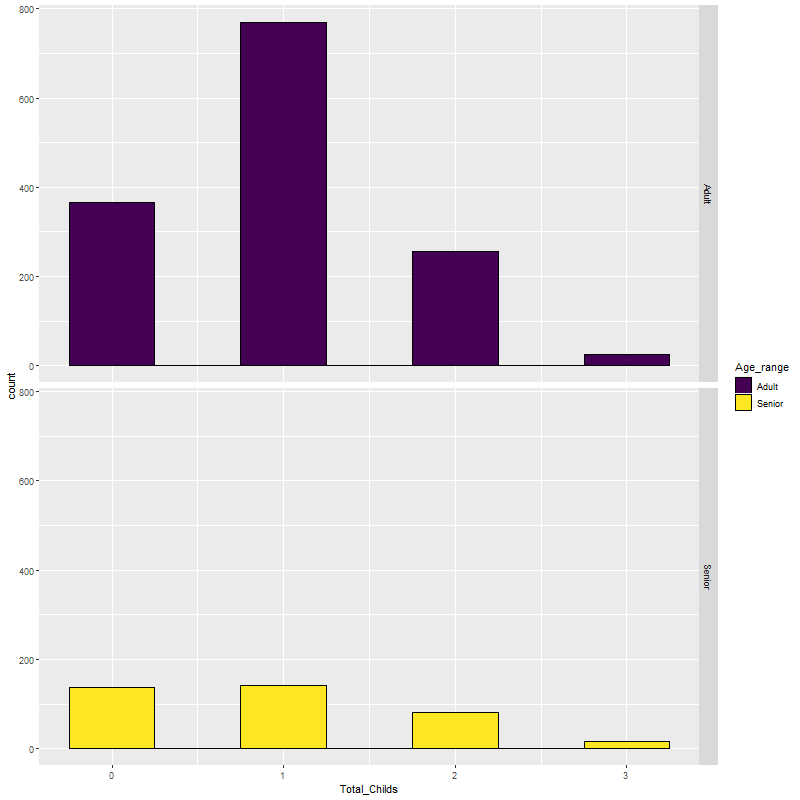
\includegraphics[width=.45\textwidth]{Img/EDA/EDA016.png}
    \caption{Istogramma di Total\_Children e Age}
    \label{fig:IstogrammaTcAge}
\end{figure}
\newpage
\paragraph{Total\_Children e Marital\_Status}
Nel pre processing i valori che può assumere la variabile \textit{Marital\_Status}sono stati collassati in due possibili valori.
\textit{Marital\_Status} è 0 se l'istanza ha come valore dell'attributo \textit{Marital\_Status} è \textit{single}, \textit{widow} oppure \textit{divorced}.
E' uguale a 1 se il valore assunto da \textit{Marital\_Status} è \textit{couple} oppure \textit{together}.
Rappresentando il diagramma a barre considerando \textit{Total\_Children}e \textit{Marital\_Status} si ricava che la maggior parte delle istanze ha un figlio. Il numero di istanze con \textit{Marital\_Status} pari a 0 è minore rispetto a quelle con valore uguale a 1 per i casi di zero e due figli, mentre per il caso di tre figli sono molto simili.


\begin{figure}[h!]
    \centering
    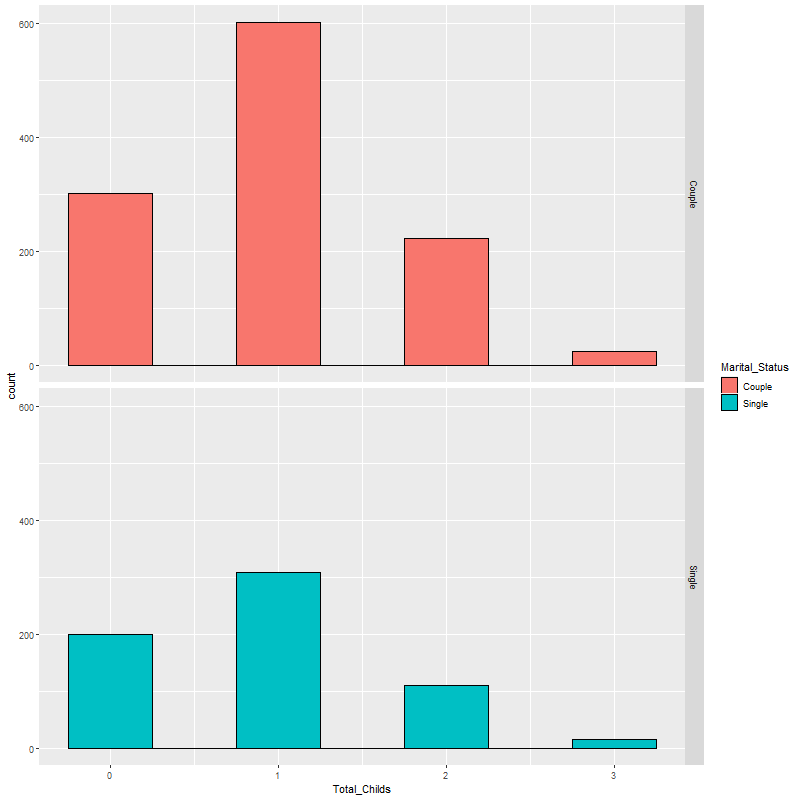
\includegraphics[width=.4\textwidth]{Img/EDA/EDA017.png}
    \caption{Istogramma di Total\_Children e Marital\_Status}
    \label{fig:IstogrammaTcMaritalStatus}
\end{figure}

Il grafico prendendo in considerazione la variabile \textit{Education} è simile. 

\begin{figure}[h!]
    \centering
    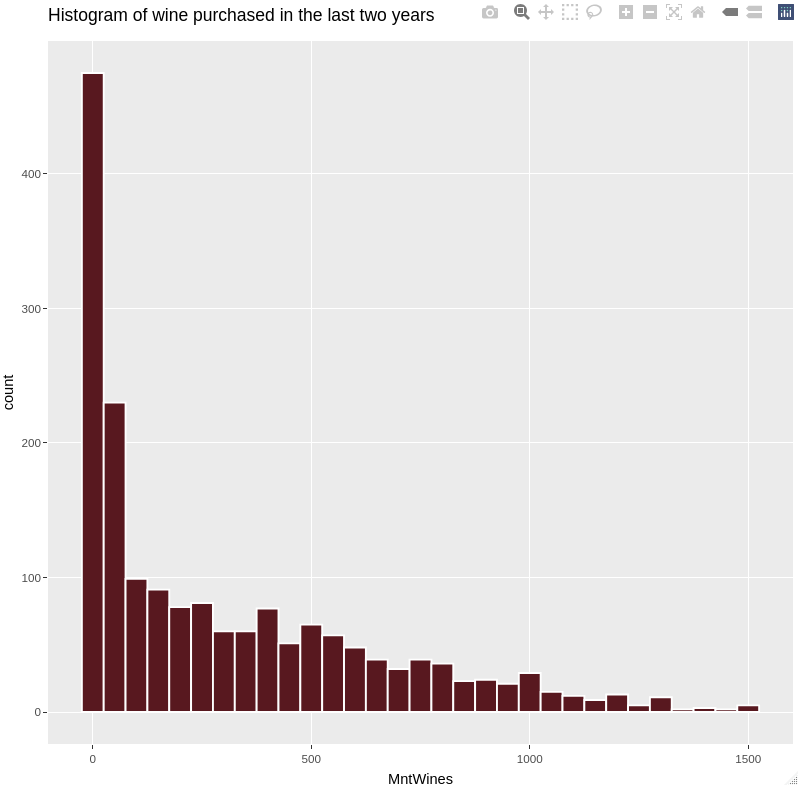
\includegraphics[width=.4\textwidth]{Img/EDA/EDA018.png}
    \caption{hist plot di Total\_Children e Education}
    \label{fig:IstogrammaTcEducation}
\end{figure}

\newpage

\paragraph{Total\_Children e Income}

Sia dall' hist plot che dal jitte rplot si nota che più è basso il guadagno più si hanno figli. Nel caso di due figli ci sono più casi di persone con stipendio \textit{low medium} rispetto a chi ha uno stipendio \textit{low}. 
Nel caso di istanze con stipendio \textit{high} è comune che si abbiano figli. 

\begin{figure}[h!]
\begin{minipage}[c]{0.4\linewidth}
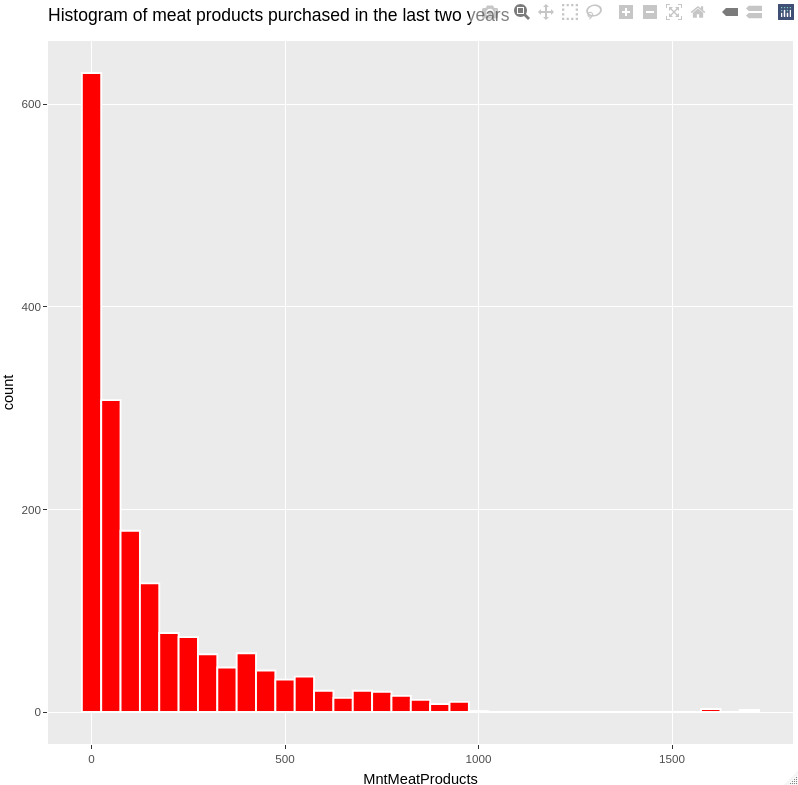
\includegraphics[width=\linewidth]{Img/EDA/EDA020.png}
\caption{Istogramma Income e Total\_Children}
\label{fig:IstogrammaTcIncome}
\end{minipage}
\hfill
\begin{minipage}[c]{0.4\linewidth}
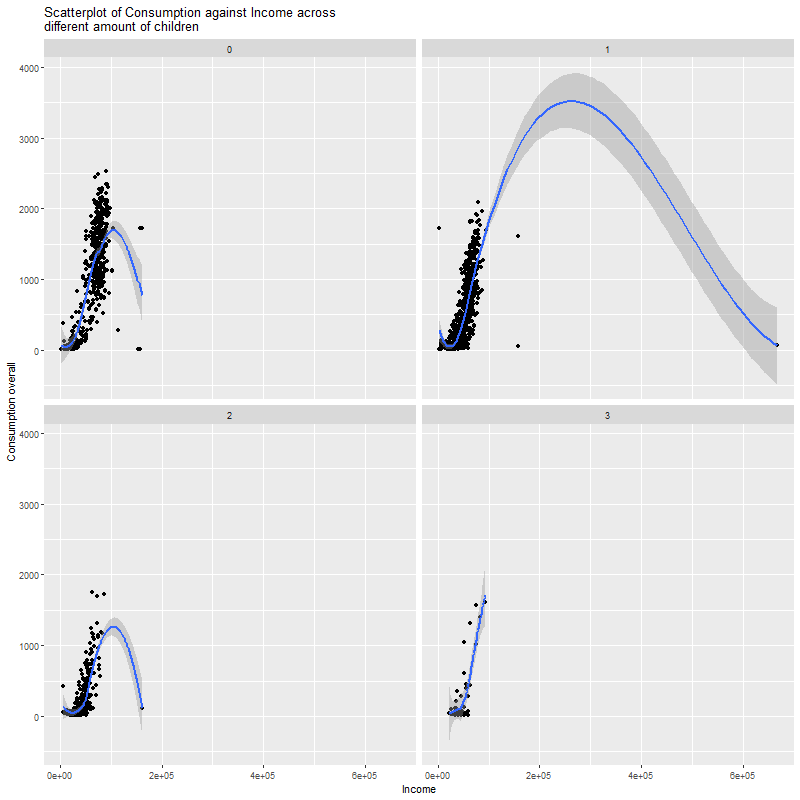
\includegraphics[width=\linewidth]{Img/EDA/EDA022.png}
\caption{ScatterPlot , Income e Total\_Children}
\label{fig:ScatterPlotTcIncome}
\end{minipage}%
\end{figure}


\begin{figure}[h!]
    \centering
    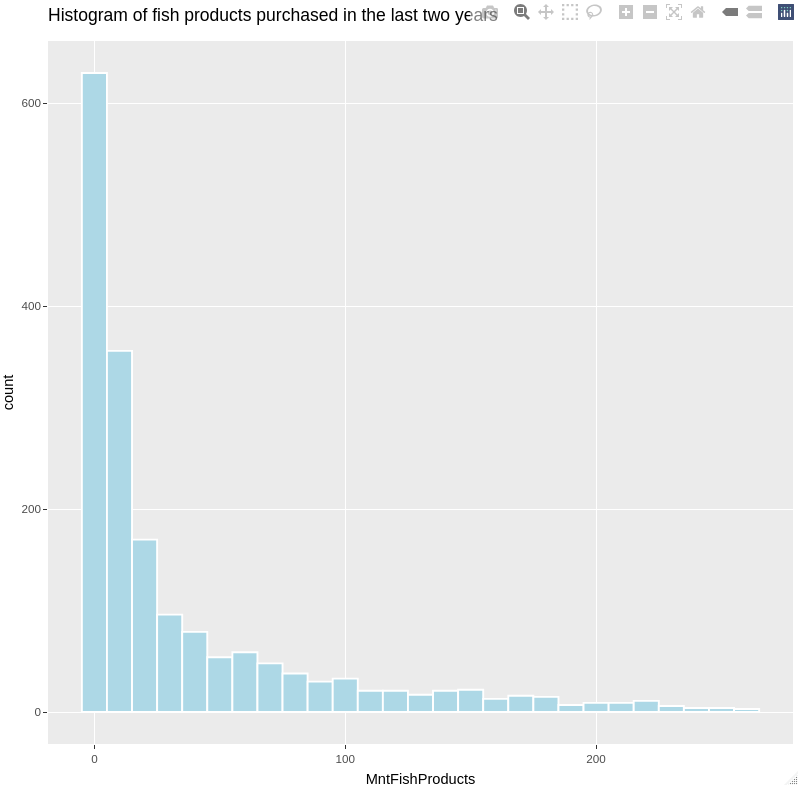
\includegraphics[width=0.5\textwidth]{Img/EDA/EDA021.png}
    \caption{JitterPlot di Total\_Children e Income}
    \label{fig:JitterPlotTcIncome}
\end{figure}

\newpage
\subsubsection{Total Spent}
La maggior parte degli individui spende meno di 500\$.
Facendo il bar-plot della variabile \textit{Total\_Spent} si nota che le istanze presenti nel dataset spendono più per il vino e per la carne.\\
Per poter produrre il grafico della Figura \ref{fig:IstogrammaTs} sono stati sommati i totali che ogni istanza ha speso per un certo prodotto.


\begin{lstlisting}[language=R]
# Plot histogram of total_spent
ggplot(trainingSet, aes(x=Total_spent)) + geom_histogram(binwidth = 15, colour = "Black")

# Create dataAcceptedCmp
dataTotalSpent <- data.frame(
  name = c("MntWines", "MntFruits", "MntMeatProducts", "MntFishProducts", "MntSweetProducts", "MntGoldProds"),  
  value = c(sum(trainingSet$MntWines), sum(trainingSet$MntFruits), sum(trainingSet$MntMeatProducts),
            sum(trainingSet$MntFishProducts), sum(trainingSet$MntSweetProducts), sum(trainingSet$MntGoldProds)))

# Barplot of total_spent for each type
ggplot(dataTotalSpent, aes(x=name, y=value)) + 
  geom_bar(stat = "identity", color = "Black") + xlab("Total Spent for each type")  
\end{lstlisting}


\begin{figure}[H]
  \centering
  \begin{minipage}[b]{0.4\textwidth}
    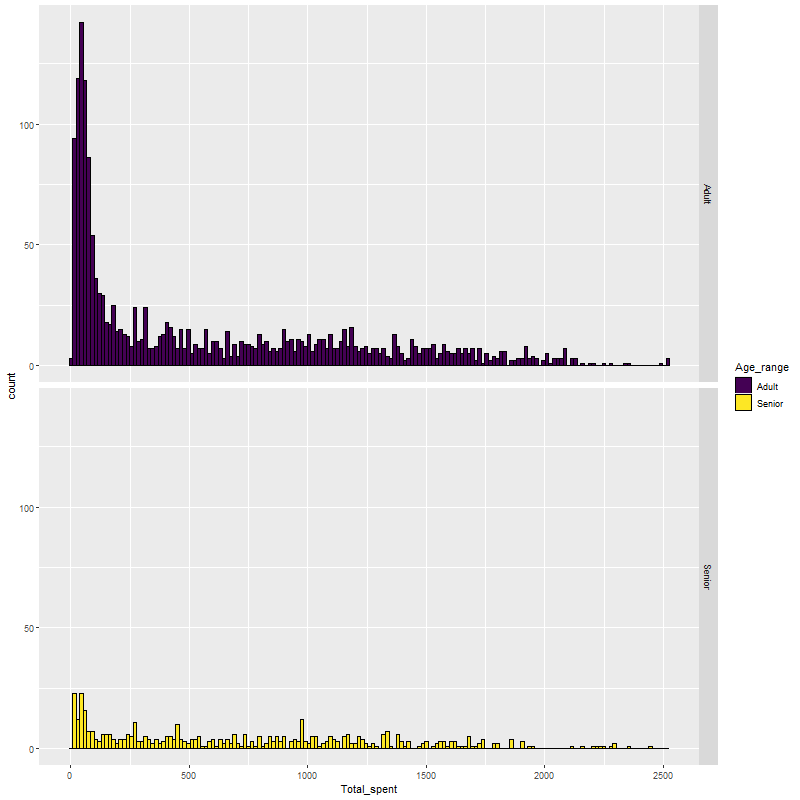
\includegraphics[width=\textwidth]{Img/EDA/EDA024.png}
    \caption{Istogramma Total\_Spent.}
    \label{fig:IstogrammaTs}
  \end{minipage}
  \hfill
  \begin{minipage}[b]{0.4\textwidth}
    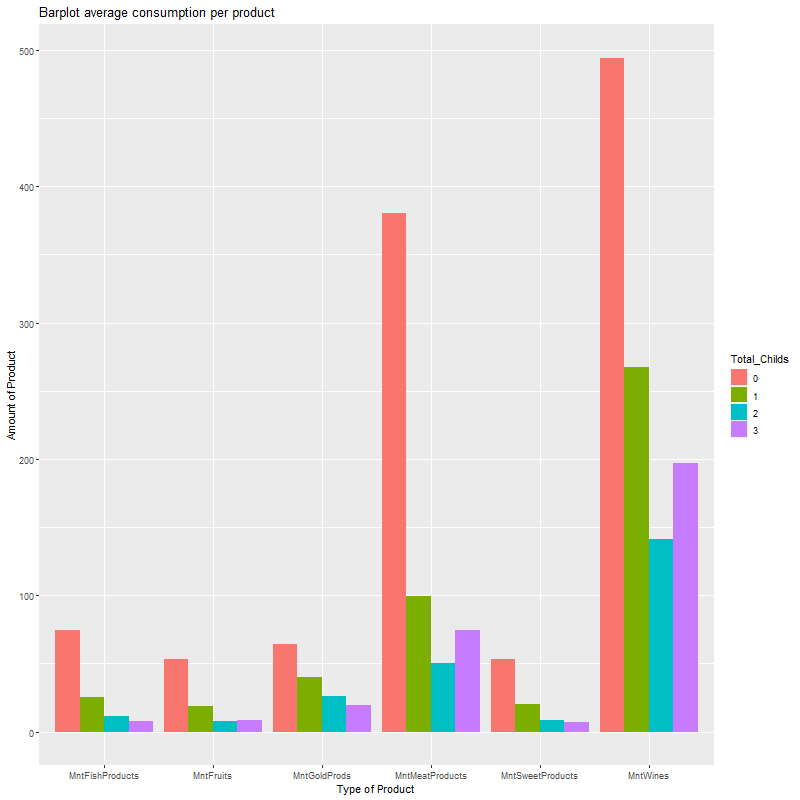
\includegraphics[width=\textwidth]{Img/EDA/EDA023.png}
    \caption{Istogramma di Total\_Spent distinguendo i tipi di prodotto.}
    \label{fig:IstogrammaTsTypeProduct}
  \end{minipage}
\end{figure}



\begin{figure}[H]
  \centering
  \begin{minipage}[b]{0.4\textwidth}
    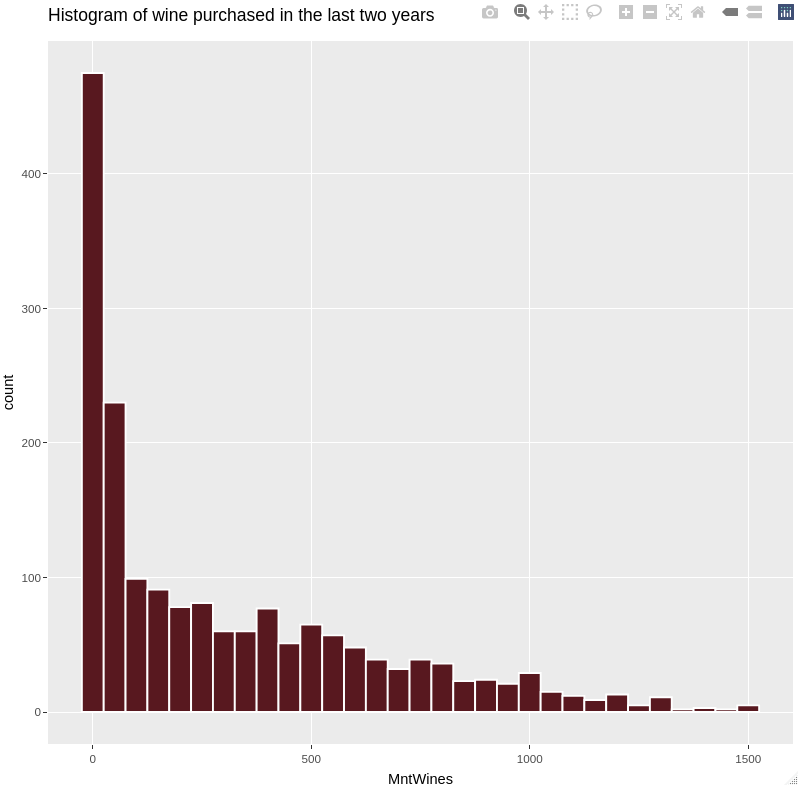
\includegraphics[width=\textwidth]{Img/EDA/EDA048.png}
    \caption{Istogramma Wine}
    \label{fig:IstogrammaWine}
  \end{minipage}
  \hfill
  \begin{minipage}[b]{0.4\textwidth}
    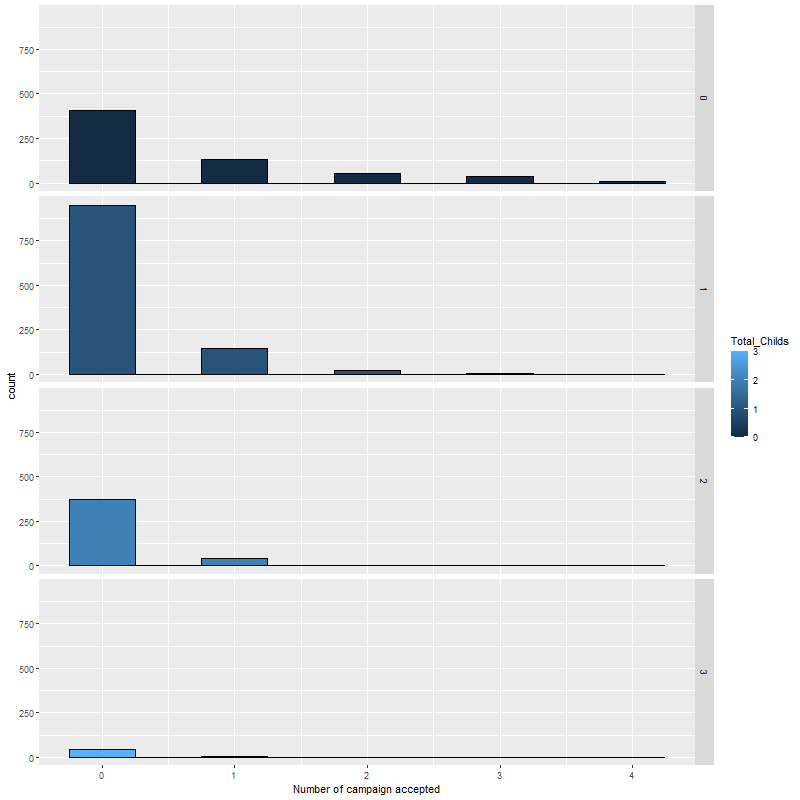
\includegraphics[width=\textwidth]{Img/EDA/EDA049.png}
    \caption{Istogramma Fruit}
     \label{fig:IstogrammaFruit}
  \end{minipage}
\end{figure}

\begin{figure}[H]
  \centering
  \begin{minipage}[b]{0.4\textwidth}
    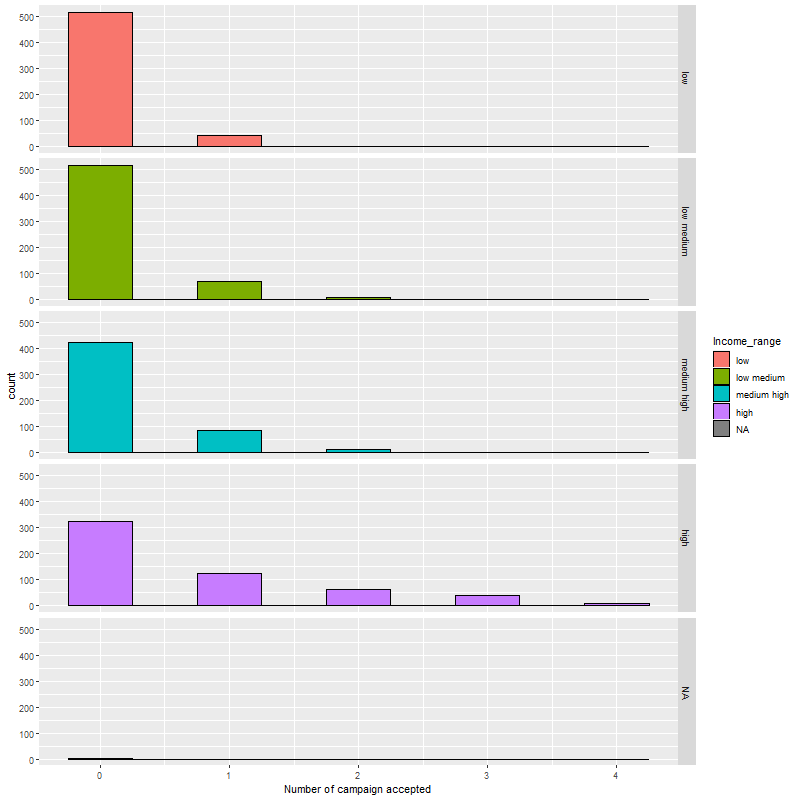
\includegraphics[width=\textwidth]{Img/EDA/EDA050.png}
    \caption{Istogramma Meat}
     \label{fig:IstogrammaMeat}
  \end{minipage}
  \hfill
  \begin{minipage}[b]{0.4\textwidth}
    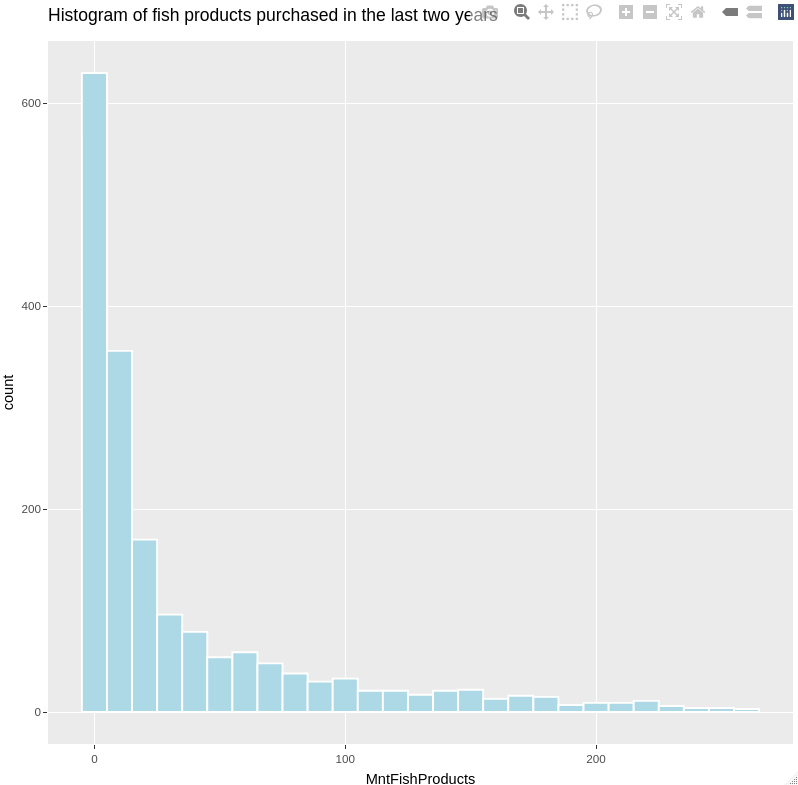
\includegraphics[width=\textwidth]{Img/EDA/EDA051.png}
    \caption{Istogramma Fish}
     \label{fig:IstogrammaFish}
  \end{minipage}
\end{figure}


\begin{figure}[H]
  \centering
  \begin{minipage}[b]{0.4\textwidth}
    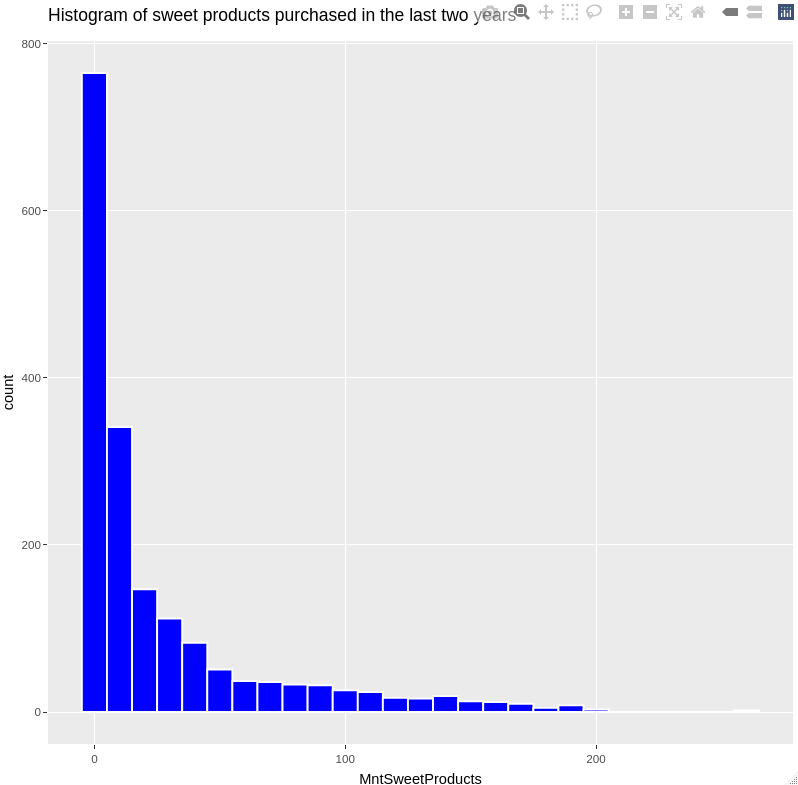
\includegraphics[width=\textwidth]{Img/EDA/EDA052.png}
    \caption{Istogramma Sweet}
     \label{fig:IstogrammaSweet}
  \end{minipage}
  \hfill
  \begin{minipage}[b]{0.4\textwidth}
    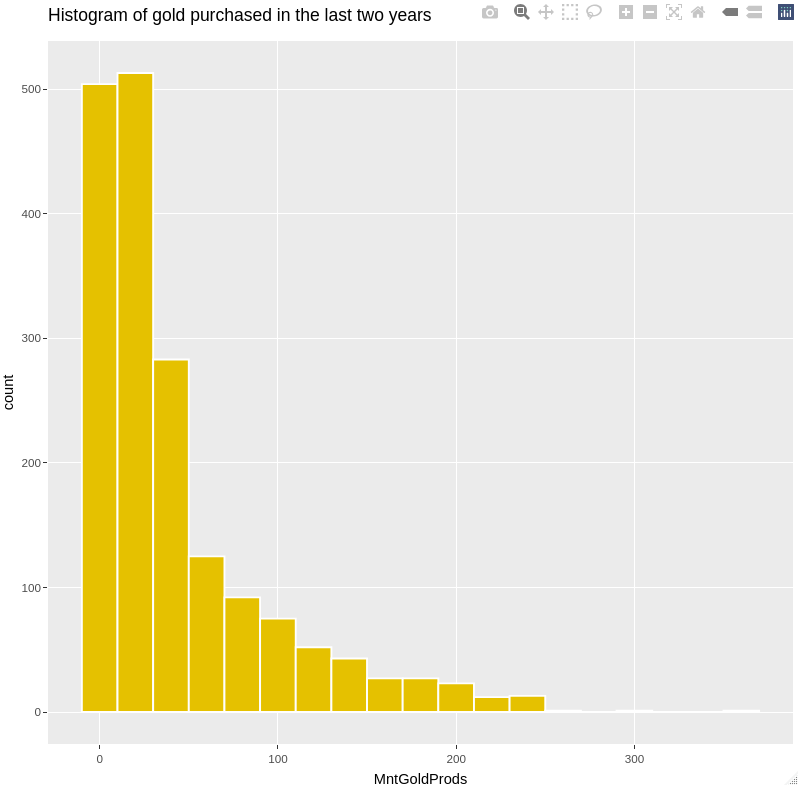
\includegraphics[width=\textwidth]{Img/EDA/EDA053.png}
    \caption{Istogramma Gold}
     \label{fig:IstogrammaGold}
  \end{minipage}
\end{figure}

\paragraph{Total Spent e Age}
Osservando la variabile \textit{Total\_Spent} considerando \textit{Age} si ha che la maggior parte degli individui spende meno di 500\$.

\begin{lstlisting}[language=R]
age_total_spent_histogram <- ggplot(trainingSet, aes(x=Total_spent)) + facet_grid(Age_range~.) 
age_total_spent_histogram + geom_histogram(aes(fill=Age_range), binwidth = 15, color="Black")
age_total_spent_histogram + geom_density(aes(fill=Age_range), position = "Stack")
\end{lstlisting}


\begin{figure}[h]
  \centering
  \begin{minipage}[b]{0.4\textwidth}
    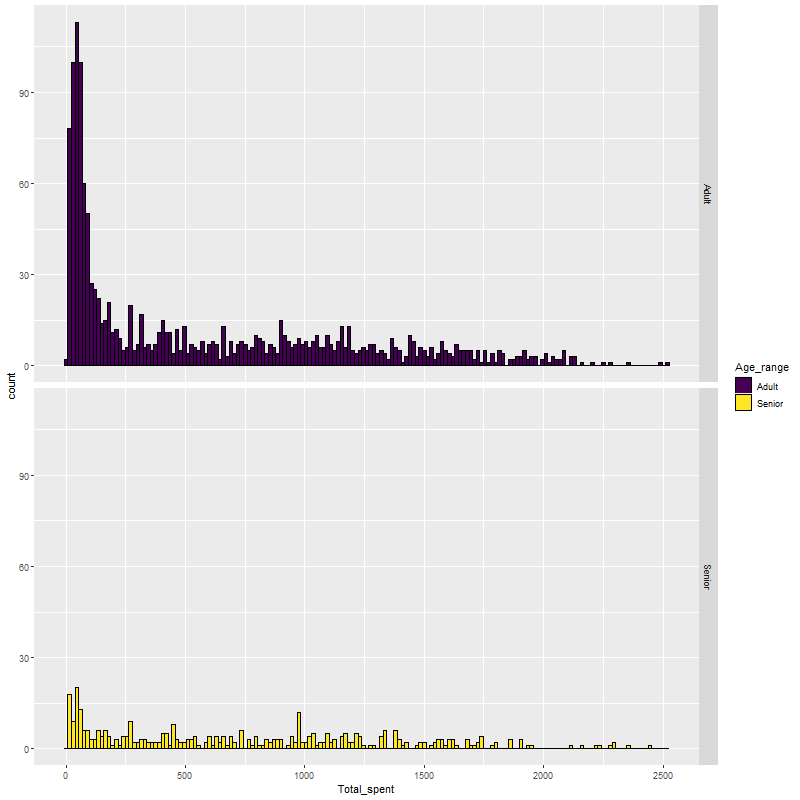
\includegraphics[width=\textwidth]{Img/EDA/EDA026.png}
    \caption{Istogramma di Total\_Spent e Age}
     \label{fig:IstogrammaTsAge}
  \end{minipage}
  \hfill
  \begin{minipage}[b]{0.4\textwidth}
    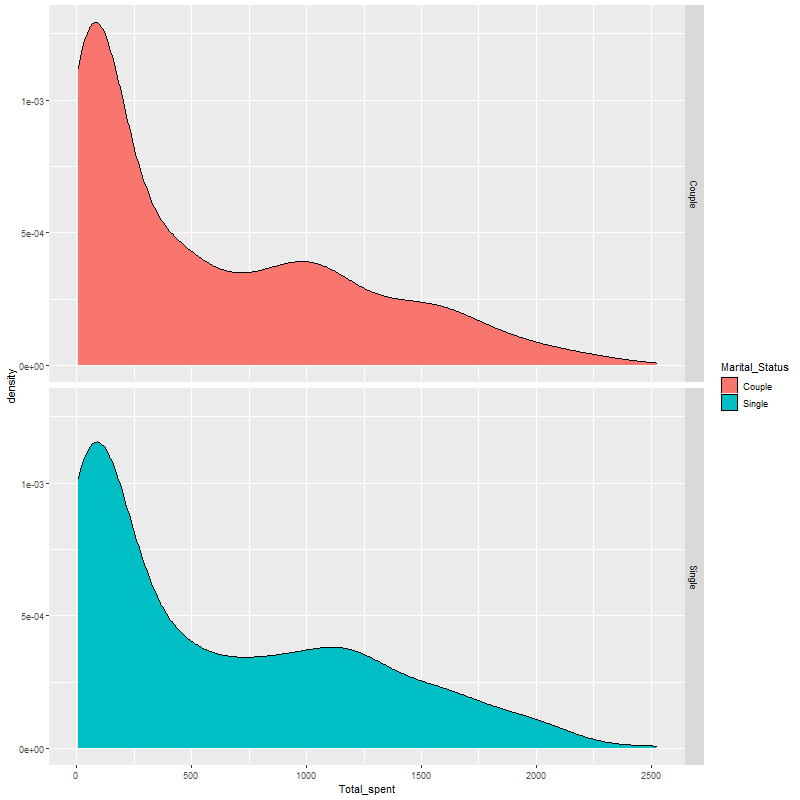
\includegraphics[width=\textwidth]{Img/EDA/EDA027.png}
    \caption{Diagramma di Densità di Total\_Spent e Age}
     \label{fig:DensitaTsAge}
  \end{minipage}
\end{figure}



\newpage
\paragraph{Total Spent e Marital\_Status}
In questo caso sembrano simili. la maggior parte delle coppie spende un totale inferiore a 500.
La situazione in single è un po' più rilassata che può essere dovuto al fatto che la maggior parte degli individui nel dataset sono coppie.

\begin{lstlisting}[language=R]
marital_status_total_spent_histogram <- ggplot(trainingSet, aes(x=Total_spent)) + facet_grid(Marital_Status~.) 
marital_status_total_spent_histogram + geom_histogram(aes(fill=Marital_Status), binwidth = 15, colour = "Black")
marital_status_total_spent_histogram + geom_density(aes(fill=Marital_Status), position = "Stack")
\end{lstlisting}


\begin{figure}[h]
  \centering
  \begin{minipage}[b]{0.4\textwidth}
    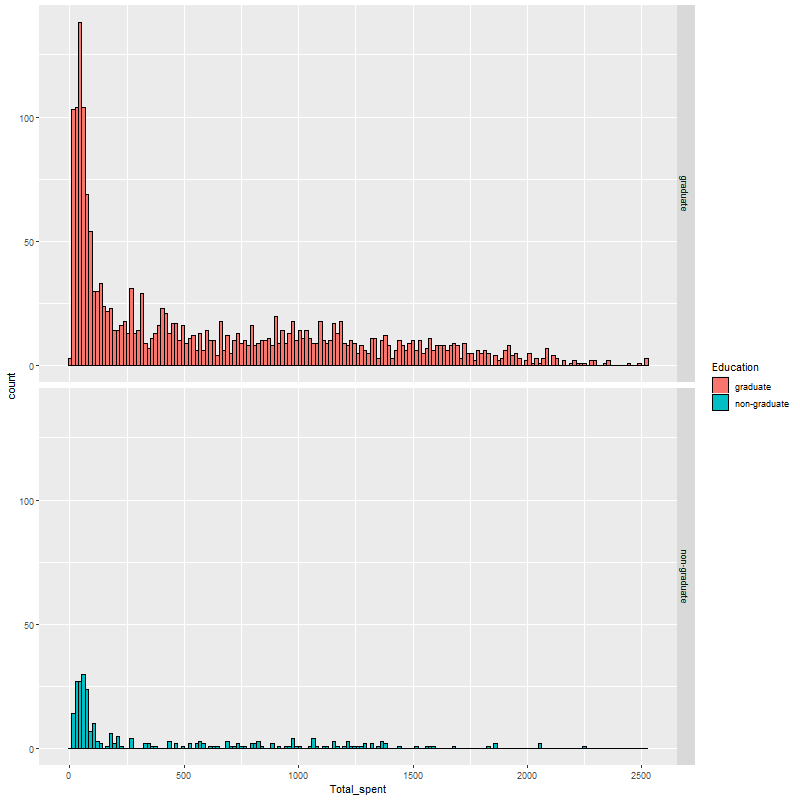
\includegraphics[width=\textwidth]{Img/EDA/EDA028.png}
    \caption{Istogramma di Total\_Spent e Marital\_Status}
    \label{fig:IstogrammaTsMaritalStatus}
  \end{minipage}
  \hfill
  \begin{minipage}[b]{0.4\textwidth}
    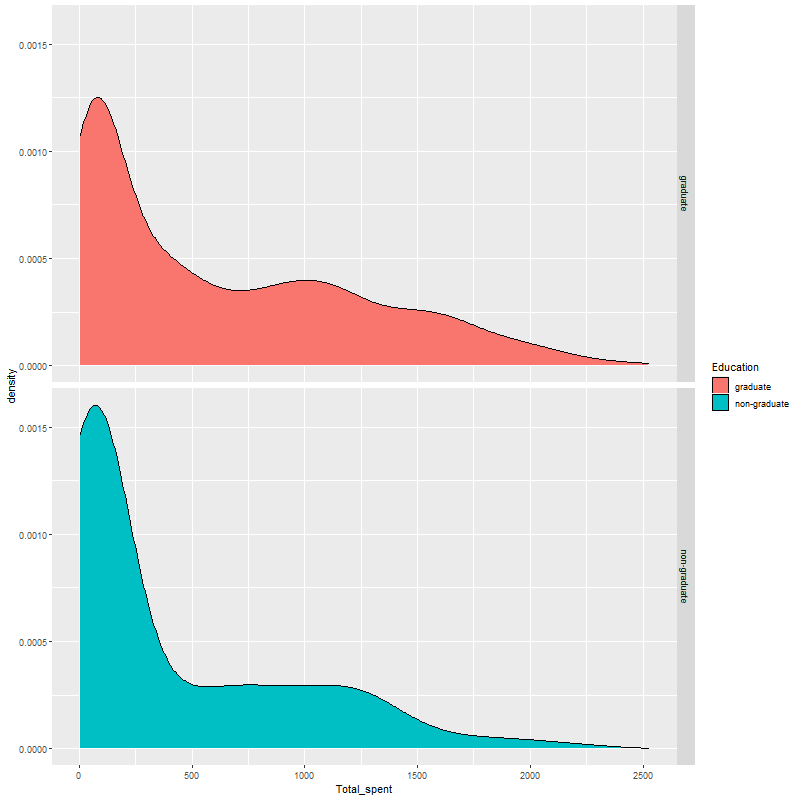
\includegraphics[width=\textwidth]{Img/EDA/EDA029.png}
    \caption{Diagramma di Densità di Total\_Spent e Marital\_Status }
     \label{fig:DensitaTsMaritalStatus}
  \end{minipage}
\end{figure}

\newpage
\paragraph{Total Spent ed Education}
I laureati in genere spendono più dei non laureati. la maggior parte dei non laureati spende da 0 a 1500. da 1500 ci sono più casi di laureati che non laureati.
Il grafico della densità   è molto simile a quello della variabile \textit{Marital\_Status}.

\begin{lstlisting}[language=R]
education_total_spent_histogram <- ggplot(trainingSet, aes(x=Total_spent)) + facet_grid(Education~.)
education_total_spent_histogram + geom_histogram(aes(fill=Education), binwidth = 15, colour = "Black")
education_total_spent_histogram + geom_density(aes(fill=Education), position = "Stack")
\end{lstlisting}


\begin{figure}[h]
  \centering
  \begin{minipage}[b]{0.4\textwidth}
    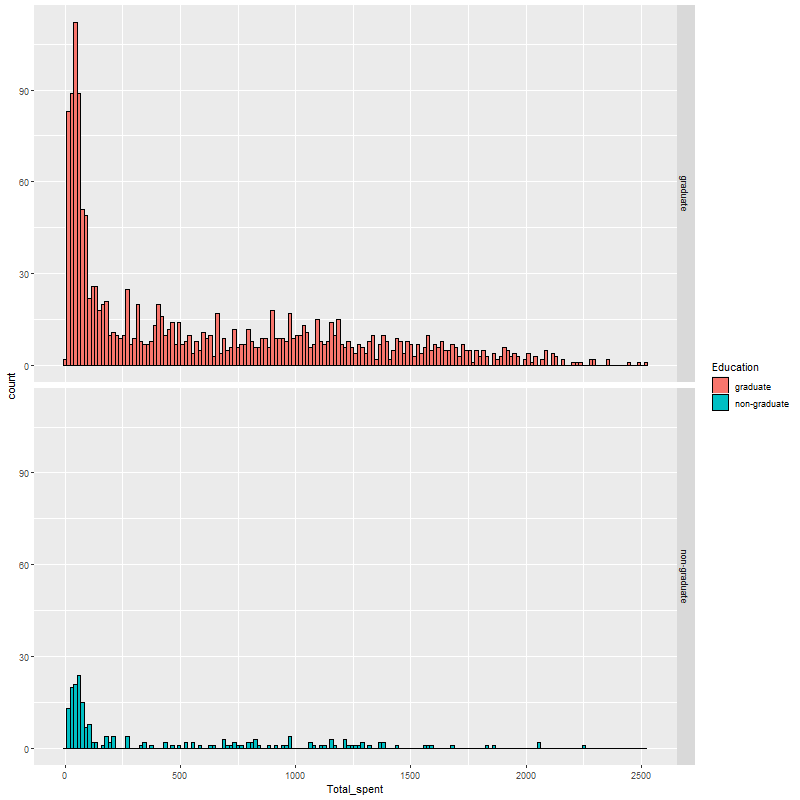
\includegraphics[width=\textwidth]{Img/EDA/EDA030.png}
    \caption{Istogramma di Total\_Spent e Education}
    \label{fig:IstogrammaTsEducation}
  \end{minipage}
  \hfill
  \begin{minipage}[b]{0.4\textwidth}
    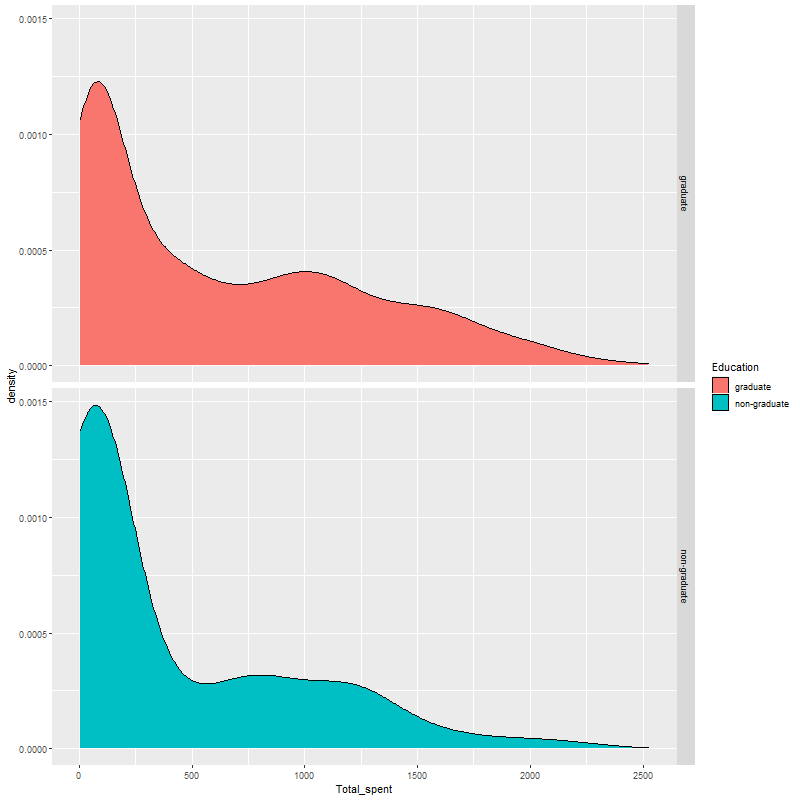
\includegraphics[width=\textwidth]{Img/EDA/EDA031.png}
    \caption{Diagramma di Densità di Total\_Spent e Education}
     \label{fig:DensitaTsEducation}
  \end{minipage}
\end{figure}


\newpage

\paragraph{Total Spent e Total\_Children}

\begin{lstlisting}[language=R]
children_total_spent_histogram <- ggplot(trainingSet, aes(x=Total_spent)) + facet_grid(Total_Childs~.)
children_total_spent_histogram  + geom_histogram(aes(fill=Total_Childs), binwidth = 15, colour = "Black")
children_total_spent_histogram  + geom_density(aes(fill=Total_Childs), position = "Stack")
\end{lstlisting}


\begin{figure}[h]
  \centering
  \begin{minipage}[b]{0.4\textwidth}
    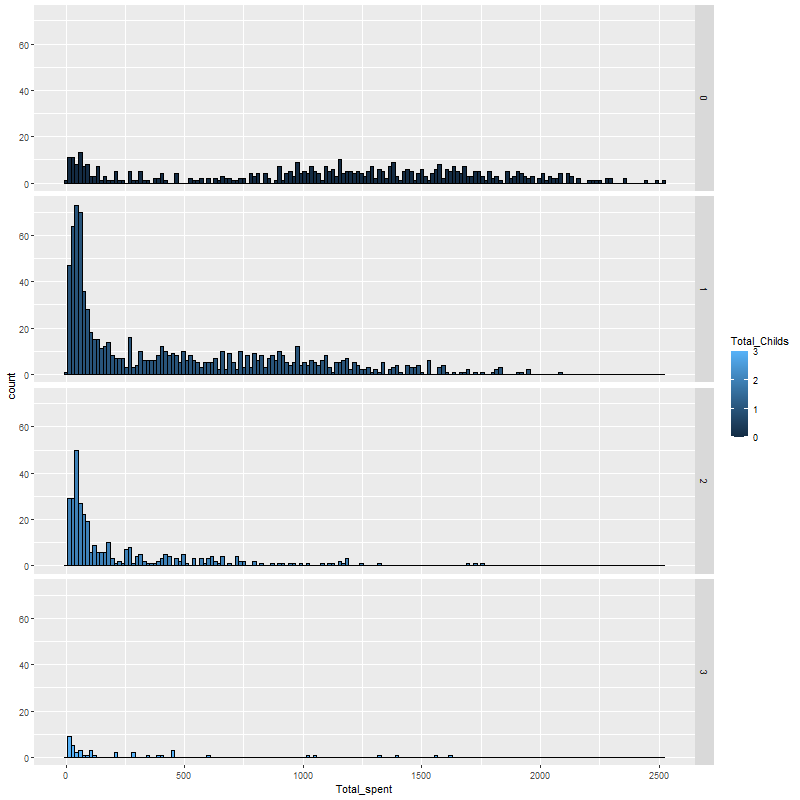
\includegraphics[width=\textwidth]{Img/EDA/EDA032.png}
    \caption{Istogramma di Total\_Spent e Total\_Children}
    \label{fig:IstogrammaTsTc}
  \end{minipage}
  \hfill
  \begin{minipage}[b]{0.4\textwidth}
    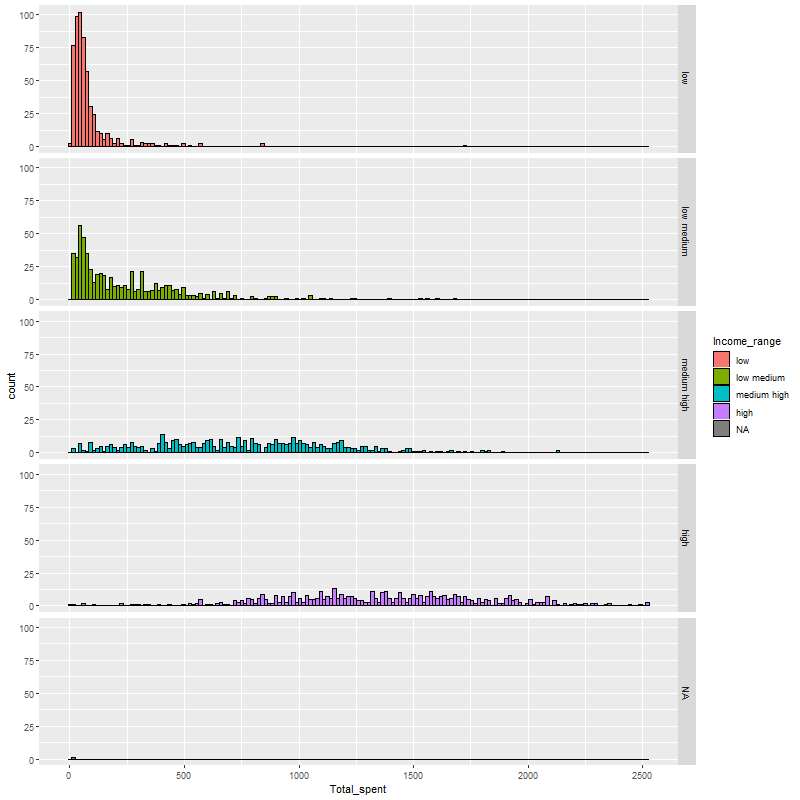
\includegraphics[width=\textwidth]{Img/EDA/EDA033.png}
    \caption{Diagramma di Densità di Total\_Spent e Total\_Children}
    \label{fig:DensitaTsTc}
  \end{minipage}
\end{figure}


\newpage
\paragraph{Total\_Spent e Income}

\begin{lstlisting}[language=R]
income_total_spent_histogram <- ggplot(trainingSet, aes(x=Total_spent)) + geom_histogram(aes(fill=Income_range), binwidth = 15, colour = "Black")
income_total_spent_histogram + facet_grid(Income_range~.)
ggplot(trainingSet, aes(y=Income, x=Total_spent)) + geom_jitter() + geom_smooth()

#--------------------------- 

ggplot(trainingSet, aes(x=Total_spent, y=Income, colour=Marital_Status, size=Income)) + 
  facet_grid(Marital_Status~Education) + 
  geom_jitter() + ylim(0,100000) + geom_smooth() + geom_boxplot(size=0.7, alpha=0.5)


ggplot(trainingSet, aes(x=Total_spent, y=Income, colour=Total_Childs, size=Income)) + 
  facet_grid(Total_Childs~Education) + 
  geom_jitter() + ylim(0,100000) + geom_smooth() + geom_boxplot(size=0.7, alpha=0.5)


ggplot(trainingSet, aes(x=Total_spent, y=Income, colour=Age_range, size=Income)) + 
  facet_grid(Age_range~Education) + 
  geom_jitter() + ylim(0,100000) + geom_smooth() + geom_boxplot(size=0.7, alpha=0.5)
\end{lstlisting}

\begin{figure}[h]
  \centering
  \begin{minipage}[b]{0.4\textwidth}
    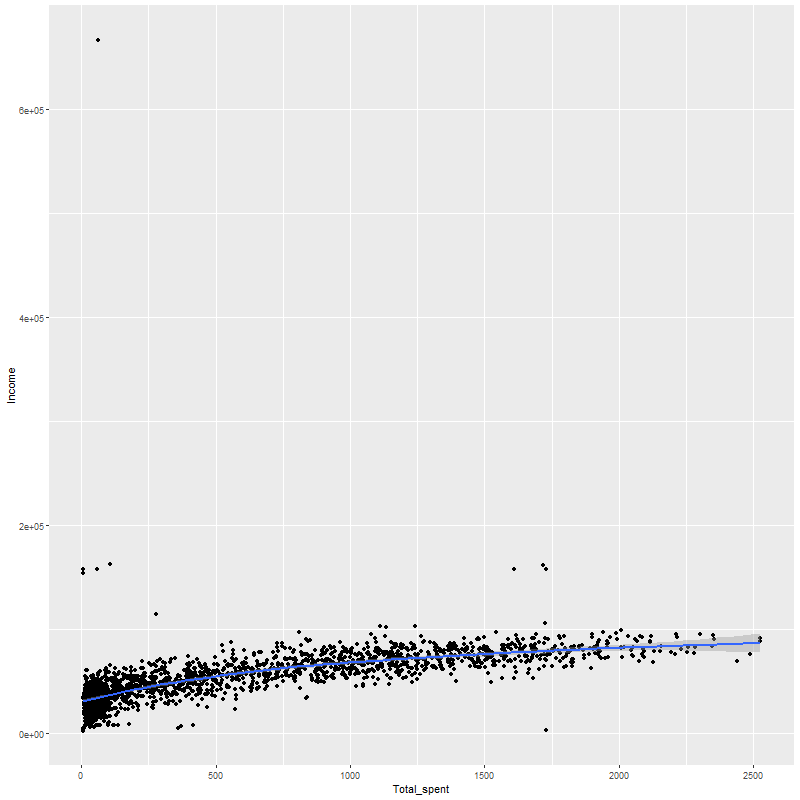
\includegraphics[width=\textwidth]{Img/EDA/EDA034.png}
    \caption{Istogramma di Total\_Spent e Income}
     \label{fig:IstogrammaTsIncome}
  \end{minipage}
  \hfill
  \begin{minipage}[b]{0.4\textwidth}
    \includegraphics[width=\textwidth]{Img/EDA/EDA035.png}
    \caption{Diagramma di Densità di Total\_Spent e Income}
     \label{fig:DensitaTsIncome}
  \end{minipage}
\end{figure}




\newpage

\begin{figure}[h]
  \centering
  \begin{minipage}[b]{0.4\textwidth}
    \includegraphics[width=\textwidth]{Img/EDA/EDA009.png}
    \caption{ScatterPlot Income e MntWines}
     \label{fig:ScatterPlotIncomeMntWines}
  \end{minipage}
  \hfill
  \begin{minipage}[b]{0.4\textwidth}
    \includegraphics[width=\textwidth]{Img/EDA/EDA010.png}
    \caption{ScatterPlot Income e MntFruits}
     \label{fig:ScatterPlotIncomeMntFruits}
  \end{minipage}
\end{figure}



\begin{figure}[h]
  \centering
  \begin{minipage}[b]{0.4\textwidth}
    \includegraphics[width=\textwidth]{Img/EDA/EDA011.png}
    \caption{ScatterPlot Income e MntMeatProducts}
     \label{fig:ScatterPlotIncomeMntMeat}
  \end{minipage}
  \hfill
  \begin{minipage}[b]{0.4\textwidth}
    \includegraphics[width=\textwidth]{Img/EDA/EDA012.png}
    \caption{ScatterPlot Income e MntFishProducts}
     \label{fig:ScatterPlotIncomeMntFish}
  \end{minipage}
\end{figure}



\paragraph{Total\_Spent JitterPlot+BoxPlot}

\begin{figure}[H]
     \begin{center}
%
        \subfigure[JitterPlot+BoxPlot di Total\_Spent, Income e Marital\_Status.]{%

            \includegraphics[width=0.5\textwidth]{Img/EDA/EDA036.png}
             \label{fig:JitterPlotTsMsIncome}
        }%
        \subfigure[JitterPlot+BoxPlot di Total\_Spent, Income e Total\_Children.]{%
            \includegraphics[width=0.5\textwidth]{Img/EDA/EDA037.png}
             \label{fig:JitterPlotTsTcIncome}
        }\\ %  ------- End of the first row ----------------------%
%
\subfigure[JitterPlot+BoxPlot di Total\_Spent, Income ed Age.]{%
            \includegraphics[width=0.5\textwidth]{Img/EDA/EDA038.png}
             \label{fig:JitterPlotTsIncomeAge}
        }\\ %  ------- End of the first row ----------------------%
%
    \end{center}
\end{figure}

\newpage

\subsubsection{Campaign Analysis}

Si è eseguita un'analisi anche sulle campagne accettate da ogni individuo. 
Per ogni istanza del dataset si sa se ha accettato o meno una campagna. In questo caso le campagne considerate sono cinque e come è possibile osservare dai barplot più di mille istanze non hanno accettato alcuna campagna, mentre chi ha accettato una o più campagne ha scelto la campagna 4.\\

\begin{figure}[H]
  \centering
  \begin{minipage}[b]{0.4\textwidth}
    \includegraphics[width=\textwidth]{Img/EDA/EDA039.png}
    \caption{Istogramma del numero totale di campagne accettate da un'istanza. Total\_Campaign}
    \label{fig:IstogrammaTotalCampaign1}
  \end{minipage}
  \hfill
  \begin{minipage}[b]{0.4\textwidth}
    \includegraphics[width=\textwidth]{Img/EDA/EDA040.png}
    \caption{Istogramma del numero di istanze che ha accettato la campagna i\-esima.}
    \label{fig:IstogrammaTotalCampaign2}
  \end{minipage}
\end{figure}

\newpage


\subsection{PCA}
La PCA è stata prevalentemente sfruttata al fine di ridurre il numero elevato di variabili che descrivono l'insieme di dati a un numero minore di variabili latenti, limitando il più possibile la perdita di informazioni. Il codice seguente mostra parte del codice riportato durante l'analisi dei dati:
\begin{lstlisting}[language=R]
pca <- PCA(trainingSet_scaled, graph = FALSE)

#Getting the variance of the first 9 new dimensions
pca$eig[,2][1:9]

#Getting the cummulative variance
pca$eig[,3][1:5]

#Getting the most correlated variables
dimdesc(pca, axes = 1:2)

# get eigenvalue
get_eigenvalue(pca)

# visualize pca
fviz_eig(pca, addlabels = TRUE, ylim = c(0, 50))
fviz_contrib(pca, choice = "var", axes = 1, top = 5)
fviz_pca_biplot(pca)

#Creating a factor map for the variable contributions
fviz_pca_var(pca, col.var = "contrib", repel = TRUE)

fviz_pca_var(pca, select.var = list(contrib = 5), col.var = "contrib", repel = TRUE)

# Extract the principal components
trainingSet_input <- data.frame(get_pca_ind(pca)$coord)
\end{lstlisting}
Da esso si vuole dare particolare attenzione alla funzione \textit{get\_eigenvalue(pca)} che fornire le informazioni rappresentate nella tabella \ref{fig:get_eigenvalue(pca)}. Si vuole anche fornire un riferimento grafico a quest'ultima tramite l'output della funzione \textit{fviz\_eig(pca, addlabels = TRUE, ylim = c(0, 50))} descritto dalla figura \ref{fig:fviz_eig(pca, addlabels = TRUE, ylim = c(0, 50))}. Da essa si può notare che le prime 5 dimensioni fornite dalla PCA forniscono il 70\% della varianza cumulativa, per questo motivo si è deciso di prendere in considerazione tali dimensioni. Inoltre si vuole sottolineare l'importanza della prima dimensione che riesce a spiegare più del 40\% della varianza dei dati.
\begin{table}[h!t]
\centering
\begin{tabular}{rrrr}
  \hline
 & eigenvalue & variance.percent & cumulative.variance.percent \\ 
  \hline
Dim.1 & 6.98 & 41.06 & 41.06 \\ 
  Dim.2 & 1.75 & 10.32 & 51.38 \\ 
  Dim.3 & 1.15 & 6.78 & 58.16 \\ 
  Dim.4 & 1.05 & 6.19 & 64.35 \\ 
  Dim.5 & 1.00 & 5.87 & 70.22 \\ 
  Dim.6 & 0.79 & 4.66 & 74.88 \\ 
  Dim.7 & 0.66 & 3.91 & 78.79 \\ 
  Dim.8 & 0.63 & 3.70 & 82.49 \\ 
  Dim.9 & 0.57 & 3.33 & 85.82 \\ 
  Dim.10 & 0.47 & 2.77 & 88.59 \\ 
  Dim.11 & 0.42 & 2.49 & 91.08 \\ 
  Dim.12 & 0.39 & 2.30 & 93.38 \\ 
  Dim.13 & 0.35 & 2.05 & 95.43 \\ 
  Dim.14 & 0.31 & 1.81 & 97.24 \\ 
  Dim.15 & 0.25 & 1.46 & 98.69 \\ 
  Dim.16 & 0.22 & 1.31 & 100.00 \\ 
  Dim.17 & 0.00 & 0.00 & 100.00 \\ 
   \hline
\end{tabular}
\caption{Output funzione \textit{get\_eigenvalue(pca)}}
\label{fig:get_eigenvalue(pca)}
\end{table}
\begin{figure}[H]
    \centering
    \includegraphics[width=0.7\textwidth]{Img/PCA/Rplot.png}
    \caption{Output funzione \textit{fviz\_eig(pca, addlabels = TRUE, ylim = c(0, 50))}}
    \label{fig:fviz_eig(pca, addlabels = TRUE, ylim = c(0, 50))}
\end{figure}
In particolare la tabella \ref{fig:pca$var$contrib} vuole far notare il contributo di ciascun attributo del dataset nella creazione delle dimensioni della pca. Da essa possiamo notare le cinque principali variabili che hanno contribuito maggiormente nella creazione della prima dimensione della \textit{principal component analysis}: Total\_spent, MntMeatProducts, NumCatalogPurchases, MntWines e MntFishProducts. La figura \ref{fig:fviz_contrib(pca, choice = "var", axes = 1, top = 5)} ne mostra un grafico più esplicativo.
\begin{figure}[H]
    \centering
    \includegraphics[width=0.7\textwidth]{Img/PCA/Rplot01.png}
    \caption{Output funzione \textit{fviz\_contrib(pca, choice = "var", axes = 1, top = 5)}}
    \label{fig:fviz_contrib(pca, choice = "var", axes = 1, top = 5)}
\end{figure}
\begin{table}[h!t]
\centering
\begin{tabular}{rrrrrr}
  \hline
 & Dim.1 & Dim.2 & Dim.3 & Dim.4 & Dim.5 \\ 
  \hline
Income & 7.31 & 0.16 & 2.59 & 3.75 & 0.92 \\ 
  Recency & 0.00 & 0.01 & 1.24 & 9.79 & 87.66 \\ 
  MntWines & 8.89 & 4.77 & 9.07 & 1.61 & 0.88 \\ 
  MntFruits & 6.99 & 1.23 & 11.85 & 0.00 & 0.35 \\ 
  MntMeatProducts & 9.55 & 1.20 & 0.11 & 0.00 & 0.12 \\ 
  MntFishProducts & 7.56 & 1.32 & 8.51 & 0.16 & 0.33 \\ 
  MntSweetProducts & 6.94 & 0.87 & 9.33 & 0.06 & 0.15 \\ 
  MntGoldProds & 4.69 & 2.38 & 6.52 & 1.19 & 0.31 \\ 
  NumDealsPurchases & 0.21 & 36.53 & 3.87 & 0.16 & 0.01 \\ 
  NumWebPurchases & 4.30 & 17.88 & 0.97 & 2.21 & 0.00 \\ 
  NumCatalogPurchases & 9.43 & 0.13 & 0.70 & 0.20 & 0.23 \\ 
  NumStorePurchases & 7.53 & 4.02 & 0.50 & 0.32 & 0.37 \\ 
  NumWebVisitsMonth & 5.78 & 8.73 & 0.35 & 12.79 & 1.36 \\ 
  Total\_spent & 13.06 & 0.49 & 0.82 & 0.58 & 0.34 \\ 
  Total\_Campains & 2.68 & 0.01 & 35.64 & 12.53 & 3.01 \\ 
  Total\_Childs & 4.79 & 14.87 & 0.20 & 2.76 & 0.15 \\ 
  Age & 0.28 & 5.40 & 7.71 & 51.88 & 3.81 \\ 
   \hline
\end{tabular}
\caption{Output \textit{pca\$var\$contrib}}
\label{fig:pca$var$contrib}
\end{table}
Le funzioni \textit{fviz\_pca\_var} hanno permesso di analizzare graficamente le dimensioni che spiegano il contributo delle variabili considerate nelle prime due dimensioni (fig. \ref{fig:fvizpcavar1} e fig. \ref{fig:fvizpcavar2}).

\begin{figure}[!htb]
   \begin{minipage}{0.48\textwidth}
     \centering
     \includegraphics[width=1\linewidth]{Img/PCA/Rplot03.png}
     \caption{Contributo di tutte la variabili sulle prime due dimensioni.}\label{fig:fvizpcavar1}
   \end{minipage}\hfill
   \begin{minipage}{0.48\textwidth}
     \centering
     \includegraphics[width=1\linewidth]{Img/PCA/Rplot04.png}
     \caption{Contributo delle cinque variabili più significative sulle prime due dimensioni.}\label{fig:fvizpcavar2}
   \end{minipage}
\end{figure}
In fine si è preso in considerazione un nuovo dataset, nato dalle dimensioni fornite dalla PCA, descritto dalla tabella \ref{fig:PCADataset}. Esso verrà sfruttato durante l'analisi del dataset tramite i diversi algoritmi utilizzati.

\begin{table}[h!t]
\centering
\begin{tabular}{rrrrrr}
  \hline
 & Dim.1 & Dim.2 & Dim.3 & Dim.4 & Dim.5 \\ 
  \hline
1 & 4.15 & 0.41 & 1.40 & 0.12 & 0.27 \\ 
  2 & -2.56 & -0.14 & -0.62 & 1.48 & -0.78 \\ 
  3 & 1.81 & -0.22 & 0.42 & 0.13 & -1.15 \\ 
  4 & -2.46 & -0.91 & 0.29 & -0.99 & -0.58 \\ 
  5 & -0.24 & 0.50 & 1.19 & 0.05 & 1.42 \\ 
  6 & 0.65 & 0.73 & -0.16 & -0.19 & -1.22 \\ 
   \hline
\end{tabular}
\caption{\textit{Head} del Dataset fornito dalla PCA}
\label{fig:PCADataset}
\end{table}


\section{Modelli utilizzati}
Il dataset non presenta una variabile target specifica, per questo motivo di è ritenuto opportuno analizzare il tutto mediante algoritmi non supervisionati come quelli di \textbf{clustering}. In particolare si è deciso di utilizzare principalmente l'algoritmo \textbf{K-Means}. Oltre a ciò si è anche cercato di trovare un target su cui poter fare predizioni mediante alberi decisionali.

\subsection{K-Means}
La natura stessa dei dati ha comportato l'obbligo di analizzare il tutto mediante un algoritmo come \textbf{K-Means}. 

\subsubsection{Silhouette e Elbow Method}
Si è ritenuto opportuno utilizzare metodi come \textbf{Elbow Method} e \textbf{Silhouette} al fine di determinare il numero ottimale di \textbf{clusters} da utilizzare. 
\begin{lstlisting}[language=R]
set.seed(6)
wcss <- vector()
for (i in 1:10) {
  wcss[i] <- sum(kmeans(trainingSet_input, i)$withinss)
}
plot(1:10, wcss, type="b", main = paste('Clusters'), xlab='Number of clusters', ylab="WCSS")


# OR

fviz_nbclust(trainingSet_input,kmeans,method="wss")+geom_vline(xintercept=2,linetype=2)
\end{lstlisting}
Il codice mostra una prima analisi mediante \textit{elbow method}, il cui output si può notare dalle figure \ref{fig:Elbow1} e \ref{fig:Elbow2}. Esse mostrano un'inclinazione tra un numero di clusters compreso tra 2 e 3.
\begin{figure}[!htb]
   \begin{minipage}{0.48\textwidth}
     \centering
     \includegraphics[width=1\linewidth]{Img/K-MEANS/KMEANS001.png}
     \caption{Elbow Method effettuato manualmente}\label{fig:Elbow1}
   \end{minipage}\hfill
   \begin{minipage}{0.48\textwidth}
     \centering
     \includegraphics[width=1\linewidth]{Img/K-MEANS/KMEANS002.png}
     \caption{Elbow Method effettuato automaticamente dal metodo $fviz\_nbclust$}\label{fig:Elbow2}
   \end{minipage}
\end{figure}
Per maggior sicurezza si è quindi deciso di sfruttare anche il metodo \textit{Silhouette} mediante il codice sottostante.

\begin{lstlisting}[language=R]
k <- 2:10
avg_sil <- sapply(k, silhouette_score)
plot(k, type='b', avg_sil, xlab='Number of clusters', ylab='Average Silhouette Scores', frame=FALSE)
avg_sil # <<<- important

# OR
fviz_nbclust(trainingSet_input, kmeans, method="silhouette")
\end{lstlisting}
Il codice presenta in output i grafici espressi delle figure \ref{fig:Silhouette1} e \ref{fig:Silhouette2}, da cui si è potuto constatare con maggior sicurezza l'utilizzo di un numero di clusters pari a 2. 
\begin{figure}[!htb]
   \begin{minipage}{0.48\textwidth}
     \centering
     \includegraphics[width=1\linewidth]{Img/K-MEANS/KMEANS003.png}
     \caption{Silhouette effettuata manualmente}\label{fig:Silhouette1}
   \end{minipage}\hfill
   \begin{minipage}{0.48\textwidth}
     \centering
     \includegraphics[width=1\linewidth]{Img/K-MEANS/KMEANS004.png}
     \caption{Silhouette effettuata automaticamente dal metodo $fviz\_nbclust$}\label{fig:Silhouette2}
   \end{minipage}
\end{figure}
\subsubsection{Algoritmo e Analisi}
Il codice sottostante viene espresso mediante le figure  \ref{fig:clusters} e \ref{fig:dissimilaritymatrix} che rappresentano rispettivamente il \textbf{partizionamento per ogni cluster} e la \textbf{Matrice di dissimilarità}. E' doveroso notare che entrambe le figure mostrano un buon partizionamento degli elementi del cluster, sebbene ci sia qualche elemento di intersezione tra i due.
\begin{lstlisting}[language=R]
set.seed(29)
km <- kmeans(trainingSet_input, 2, nstart = 10)
print(km$centers)
fviz_cluster(km, trainingSet_input, geom = "point",ellipse.type = "norm",repel = TRUE)
cl <- km$cluster
dissplot(dist(trainingSet_input), labels=cl,options=list(main="Kmeans Clustering With k=2"))
\end{lstlisting}

\begin{figure}[!htb]
   \begin{minipage}{0.48\textwidth}
     \centering
         \includegraphics[width=1\textwidth]{Img/K-MEANS/KMEANS005.png}
    \caption{Partizionamento in clusters dei dati}
    \label{fig:clusters}
   \end{minipage}\hfill
   \begin{minipage}{0.48\textwidth}
     \centering
     \includegraphics[width=1\linewidth]{Img/K-MEANS/KMEANS006.png}
     \caption{Dissimilarity matrix}\label{fig:dissimilaritymatrix}
   \end{minipage}
\end{figure}
In particolare la figura \ref{fig:clusters} presenta gli elementi all'interno di ogni cluster. La tabella \ref{fig:clustersnumberelements} mostra il numero preciso di elementi per ogni cluster.
\begin{table}[h!t]
\centering
\begin{tabular}{rlr}
  \hline
 & cluster & n \\ 
  \hline
1 & 1 & 1081 \\ 
  2 & 2 & 711 \\ 
   \hline
\end{tabular}
\caption{Numero di elementi per ogni cluster}
\label{fig:clustersnumberelements}
\end{table}
Si è ritenuto necessario analizzare i risultati ottenuti mediante le variabili più significative, sorte durante la \textit{Principal Component Analisys}. 
\begin{lstlisting}[language=R]
wines <- ggplot(trainingSet, aes(MntWines)) + 
   facet_grid(cluster~.) 

wines + geom_histogram(color = "black", fill = "red") 
wines + geom_density(fill="red", position = "Stack")
ggplot(trainingSet, aes(x=cluster,y=MntWines,fill=cluster))+geom_boxplot(outlier.colour="black")
\end{lstlisting}
Il codice soprastante è descritto dalle figure \ref{fig:winesKmeansBoxPlot}, \ref{fig:winesKmeansDensity} e \ref{fig:winesKmeansHistogram}. Dall'analisi dei grafici si nota una spesa maggiore di vini per i \textit{customers} all'interno del secondo cluster. In particolare la maggior parte dei clienti all'interno del primo cluster non ha acquistato vini negli ultimi due anni. 

\begin{figure}[!htb]
   \begin{minipage}{0.48\textwidth}
     \centering
         \includegraphics[width=1\textwidth]{Img/K-MEANS/KMEANS007.png}
    \caption{Istogramma della variabile Wines in relazione al numero di cluster}
    \label{fig:winesKmeansHistogram}
   \end{minipage}\hfill
   \begin{minipage}{0.48\textwidth}
     \centering
     \includegraphics[width=1\linewidth]{Img/K-MEANS/KMEANS008.png}
     \caption{Diagramma di densità della variabile Wines in relazione al numero di cluster}\label{fig:winesKmeansDensity}
   \end{minipage}
\end{figure}

\begin{figure}[H]
    \centering
    \includegraphics[width=0.7\textwidth]{Img/K-MEANS/KMEANS009.png}
    \caption{BoxPlot della variabile Wines in relazione al numero di cluster}
    \label{fig:winesKmeansBoxPlot}
\end{figure}

\begin{lstlisting}[language=R]
income <- ggplot(trainingSet, aes(Income))+ 
  facet_grid(cluster~.) + 
  xlim(0,200000)

income +  geom_histogram(color = "black", fill = "green")
income + geom_density(fill="green", position = "Stack")
ggplot(trainingSet, aes(x=cluster,y=Income,fill=cluster))+geom_boxplot(outlier.colour="black") + ylim(0,200000)
\end{lstlisting}
Il codice appena descritto ha il compito di analizzare gli elementi dei cluster in relazione al reddito di ciascun utente, ovvero in relazione alla variabile \textit{income}. Le figure \ref{fig:incomeKmeansDensity}, \ref{fig:incomeKmeansHistogram} e \ref{fig:incomeKmeansBoxPlot} ne mostrano la rappresentazione dei grafici. Da esse è doverso notare che nel primo cluster la maggior parte dei clienti possiede un reddito generalmente più basso rispetto ai \textit{customers} facenti parte del secondo. Calcolando il reddito medio dei compratori, pari a 52247 dollari, si può anche notare che la maggior parte degli elementi nel primo cluster possiedono un il reddito inferiore alla media. E' opportuno notare anche che, la maggior parte degli utenti del secondo cluster, contrariamente ai primi, possiedono un reddito superiore alla media.

\begin{figure}[!htb]
   \begin{minipage}{0.48\textwidth}
     \centering
         \includegraphics[width=1\textwidth]{Img/K-MEANS/KMEANS010.png}
    \caption{Istogramma della variabile Income in relazione al numero di cluster}
    \label{fig:incomeKmeansHistogram}
   \end{minipage}\hfill
   \begin{minipage}{0.48\textwidth}
     \centering
     \includegraphics[width=1\linewidth]{Img/K-MEANS/KMEANS011.png}
     \caption{Diagramma di densità della variabile Income in relazione al numero di cluster}\label{fig:incomeKmeansDensity}
   \end{minipage}
\end{figure}

\begin{figure}[H]
    \centering
    \includegraphics[width=0.7\textwidth]{Img/K-MEANS/KMEANS012.png}
    \caption{BoxPlot della variabile income in relazione al numero di cluster}
    \label{fig:incomeKmeansBoxPlot}
\end{figure}

Un'altra variabile analizzata è Total\_spent, che spiega la gran parte della varianza della prima dimensione della PCA. Il codice sottostante speiga le figure \ref{fig:TotalSpentKmeansBoxPlot}, \ref{fig:TotalSpentKmeansDensity} e \ref{fig:TotalSpentKmeansHistogram}. In particolare, dall'analisi di esse è emerso che i compratori del primo cluster generalmente molto meno denaro rispetto a quelli del secondo. Oltre a ciò si può anche notare che quest'ultimi spendono mediamente più di mille dollari ogni due anni per prodotti come: vino, frutta, pesce e carne.
\begin{lstlisting}[language=R]
ts <- ggplot(trainingSet, aes(Total_spent), colour=cluster) + facet_grid(cluster~.)
ts + geom_histogram(color = "black", fill = "purple") 
ts + geom_density(fill="purple", position = "Stack")
ggplot(trainingSet, aes(x=cluster,y=Total_spent,fill=cluster))+geom_boxplot(outlier.colour="black")
\end{lstlisting}
\begin{figure}[!htb]
   \begin{minipage}{0.48\textwidth}
     \centering
         \includegraphics[width=1\textwidth]{Img/K-MEANS/KMEANS013.png}
    \caption{Istogramma della variabile Total\_spent in relazione al numero di cluster}
    \label{fig:TotalSpentKmeansHistogram}
   \end{minipage}\hfill
   \begin{minipage}{0.48\textwidth}
     \centering
     \includegraphics[width=1\linewidth]{Img/K-MEANS/KMEANS014.png}
     \caption{Diagramma di Densità della variabile Total\_spent in relazione al numero di cluster}\label{fig:TotalSpentKmeansDensity}
   \end{minipage}
\end{figure}

\begin{figure}[H]
    \centering
    \includegraphics[width=0.7\textwidth]{Img/K-MEANS/KMEANS015.png}
    \caption{BoxPlot della variabile Total\_spent in relazione al numero di cluster}
    \label{fig:TotalSpentKmeansBoxPlot}
\end{figure}

Le figure \ref{fig:NumCatalogPurchasesKmeansBoxPlot}, \ref{fig:NumCatalogPurchasesKmeansDensity} e \ref{fig:NumCatalogPurchasesKmeansHistogram} mostrano che i clienti del primo cluster effettuino compere sul catalogo generalmente in quantità minore rispetto a quelli del secondo. Difatti ques'ultimi acquistano mediamente 5 prodotti dal catalogo.
\begin{lstlisting}[language=R]
numCatalogPurchases <- ggplot(trainingSet, aes(NumCatalogPurchases)) +  facet_grid(cluster~.)
numCatalogPurchases + geom_histogram(color = "black", fill = "blue") 
numCatalogPurchases + geom_density(fill="blue", position = "Stack")
ggplot(trainingSet, aes(x=cluster,y=NumCatalogPurchases,fill=cluster))+geom_boxplot(outlier.colour="black") + ylim(0,10)
\end{lstlisting}

\begin{figure}[!htb]
   \begin{minipage}{0.48\textwidth}
     \centering
         \includegraphics[width=1\textwidth]{Img/K-MEANS/KMEANS016.png}
    \caption{Istogramma della variabile NumCatalogPurchases in relazione al numero di cluster}
    \label{fig:NumCatalogPurchasesKmeansHistogram}
   \end{minipage}\hfill
   \begin{minipage}{0.48\textwidth}
     \centering
     \includegraphics[width=1\linewidth]{Img/K-MEANS/KMEANS017.png}
     \caption{Diagramma di Densità della variabile NumCatalogPurchases in relazione al numero di cluster}\label{fig:NumCatalogPurchasesKmeansDensity}
   \end{minipage}
\end{figure}

\begin{figure}[H]
    \centering
    \includegraphics[width=0.7\textwidth]{Img/K-MEANS/KMEANS018.png}
    \caption{BoxPlot della variabile NumCatalogPurchases in relazione al numero di cluster}
    \label{fig:NumCatalogPurchasesKmeansBoxPlot}
\end{figure}

Dall'analisi della variabile \textit{MntMeatProducts}, inerente all'acquisto di prodotti di carne negli ultimi due anni, si possono evincere alcune importanti informazioni correlate anche alla precedente analisi di \textit{Total\_spent}. In particolare le figure \ref{fig:MntMeatProductsKmeansBoxPlot}, \ref{fig:MntMeatProductsKmeansDensity} e \ref{fig:MntMeatProductsKmeansHistogram} mostrano come gli acquirenti del primo cluster tendano a spendere generalmente di meno rispetto a quelli del secondo. Difatti i primi acquistano sicuramente molto meno rispetto alla media di circa 170 dollari ogni due anni spesi per prodotti di carne.

\begin{lstlisting}[language=R]
meat <- ggplot(trainingSet, aes(MntMeatProducts)) +  facet_grid(cluster~.)
meat + geom_histogram(color = "black", fill = "brown") 
meat + geom_density(fill="brown", position = "Stack")
ggplot(trainingSet, aes(x=cluster,y=MntMeatProducts,fill=cluster))+geom_boxplot(outlier.colour="black")
\end{lstlisting}


\begin{figure}[!htb]
   \begin{minipage}{0.48\textwidth}
     \centering
         \includegraphics[width=1\textwidth]{Img/K-MEANS/KMEANS019.png}
    \caption{Istogramma della variabile MntMeatProducts in relazione al numero di cluster}
    \label{fig:MntMeatProductsKmeansHistogram}
   \end{minipage}\hfill
   \begin{minipage}{0.48\textwidth}
     \centering
     \includegraphics[width=1\linewidth]{Img/K-MEANS/KMEANS020.png}
     \caption{Diagramma di Densità della variabile MntMeatProducts in relazione al numero di cluster}\label{fig:MntMeatProductsKmeansDensity}
   \end{minipage}
\end{figure}

\begin{figure}[H]
    \centering
    \includegraphics[width=0.7\textwidth]{Img/K-MEANS/KMEANS021.png}
    \caption{BoxPlot della variabile MntMeatProducts in relazione al numero di cluster}
    \label{fig:MntMeatProductsKmeansBoxPlot}
\end{figure}


\newpage
\subsection{D-Tree}
Usando il dataset ricavato dalla PCA ovvero \textit{trainingSet\_input} si è cercato di fare una previsione sul valore che assume la variabile \textit{Response}. Per farlo è stata aggiunta una variabile al dataset. 

\begin{lstlisting}[language=R]
trainingSet_input$Response<-trainingSet$Response
\end{lstlisting}

Successivamente è stata usata la funzione \textit{rpart} per costruire un albero di decisione indicando come formula la variabile \textit{Response}.

\begin{lstlisting}[language=R]
response.default.tree <- rpart(Response ~ ., data = trainingSet_input, method = "class")
\end{lstlisting}

Per visualizzarlo si è eseguita la funzione prp del \textit{package, rpart.plot} indicando per i campi richiesti un parametro come per esempio \textit{type} che assegna a tutti i nodi un etichetta, non solo le foglie. \textit{extra}, che se uguale ad 1 visualizza il numero di osservazioni che cadono nel nodo. 

\begin{lstlisting}[language=R]
prp(response.default.tree, 
     type = 1, extra = 1, varlen = -10, 
     box.col = ifelse(customer.default.tree$frame$var == "<leaf>", 'gray', 'white'))
\end{lstlisting}

\begin{figure}[H]
    \centering
    \includegraphics[width=0.6\textwidth]{Img/D-TREE/D-TREE001.png}
    \caption{DecisionTree response.default.tree}
\end{figure}


Successivamente si è eseguita una previsione sulla variabile \textit{Response} tramite la funzione \textit{predict} passando come parametro anche l'albero \textit{response.default.tree}. 

\begin{lstlisting}[language=R]
response.default.tree.pred <- predict(response.default.tree, trainingSet_input,type = "class")
\end{lstlisting}

Per confrontare il valore effetivo della variabile \textit{Response} e della previsione si è fatta la matrice di confusione. 

\begin{lstlisting}[language=R]
confusionMatrix.default<-confusionMatrix(response.default.tree.pred, as.factor(trainingSet_input$Response), positive = "1")
\end{lstlisting}



\begin{table}[h!]
\centering
\begin{tabular}{|ll|lll|}
\hline
\multicolumn{2}{|l|}{\multirow{2}{*}{}} & \multicolumn{3}{l|}{Reference}                        \\ \cline{3-5} 
\multicolumn{2}{|l|}{}                  & \multicolumn{1}{c|}{\_} & \multicolumn{1}{l|}{0}  & 1  \\ \hline
\multicolumn{2}{|l|}{\multirow{2}{*}{Prediction}} & \multicolumn{1}{l|}{0} & \multicolumn{1}{l|}{1515} & 196 \\ \cline{3-5} 
\multicolumn{2}{|l|}{}                  & \multicolumn{1}{l|}{1} & \multicolumn{1}{l|}{10} & 71 \\ \hline
\end{tabular}
\end{table}

Dalla matrice di confusione sommando i valori presenti nella diagonale e facendo il rapporto con la somma di tutti i valori della matrice si ricava che l'accuratezza è del 88.5\%.
Si può ricavare anche la precisione che è pari al rapporto tra il numero di istanze   classificate con il valore 1 e che corrisponde al valore che ha \textit{Response} e il numero di istanze classificate con il valore 1 al 87.6\%.
Di seguito sono riportati altri dati statistici che è possibile ricavare. 

\begin{table}[h!]
\centering
\begin{tabular}{ll}
\multicolumn{2}{l}{\textbf{Positive Class:} 1}          \\
\textbf{Sensitivity:} 0.26592 & \textbf{Pos Pred Value:} 0.87654 \\
\textbf{Specificity:} 0.99344 & \textbf{Neg Pred Value:} 0.88545
\end{tabular}
\end{table}

Per capire meglio l'albero decisionale si usa la funzione printcp().

\begin{lstlisting}[language=R]
cv.ct <- rpart( Response ~ ., data = trainingSet_input, method ="class", cp = 0, minsplit = 2, xval = 10)
printcp(cv.ct)
\end{lstlisting}

\textbf{Variables actually used in tree construction:} Dim.1 Dim.2 Dim.3 Dim.4 Dim.5\\
\textbf{Root node error:} 267/1792 = 0.149\\
\textbf{n=}1792 

\begin{table}[ht]
\centering
\begin{tabular}{rrrrrr}
  \hline
 & CP & nsplit & rel error & xerror & xstd \\ 
  \hline
1 & 0.0880150 & 0 & 0.00000 & 1.00000 & 0.056456 \\ 
  2 & 0.0131086 & 2 & 0.823970 & 0.84270 & 0.052535 \\ 
  3 & 0.0074906 & 6 & 0.771536 & 0.85393 & 0.052833 \\ 
  4 & 0.0056180 & 9 & 0.749064 & 0.91386 & 0.054375 \\ 
  5 & 0.0049938 & 32 & 0.554307 & 0.91386 & 0.054375 \\ 
  6 & 0.0037453 & 38 & 0.524345 & 0.91386 & 0.054375 \\ 
  7 & 0.0028090 & 98 & 0.299625 & 0.99625 & 0.056369 \\ 
  8 & 0.0024969 & 114 & 0.250936 & 1.04494 & 0.057483 \\ 
  9 & 0.0022472 & 123 & 0.228464 & 1.04494 & 0.057483 \\ 
  10 & 0.0018727 & 128 & 0.217228 & 1.11236 & 0.058955 \\ 
  11 & 0.0012484 & 202 & 0.052434 & 1.11236 & 0.058955 \\ 
  12 & 0.000000 & 205 & 0.048689 & 1.11985 & 0.059113 \\ 
   \hline
\end{tabular}
\end{table}

Succesivamente si è cercato il miglior albero di decisione prendendo prima il minimo tra una matrice di informazioni sulle strutture ottimali in base ad un parametro di complessità, cp dalla\textit{cptable} che è pari a 0.8426966.
Poi si è cercato l'errore standard corrispondente al minimo errore che è 0.05253461.  

\begin{lstlisting}[language=R]
# min error
minerror <- min(cv.ct$cptable[ , 4])
minerror

minerrorstd <- cv.ct$cptable[cv.ct$cptable[,4] == minerror, 5]
minerrorstd
\end{lstlisting}

\begin{lstlisting}[language=R]
# set of trees where xerror is less than minerror + minerrorstd
simplertrees <- cv.ct$cptable[cv.ct$cptable[,4] < minerror + minerrorstd, ]
simplertrees
\end{lstlisting}


\begin{lstlisting}[language=R]
# cp of the simplest of those trees
bestcp <- simplertrees[1, 1]
bestcp
\end{lstlisting}
\begin{table}[ht]
\centering
\begin{tabular}{rrrrrr}
  \hline
 & CP & nsplit & rel error & xerror & xstd \\ 
  \hline
  2 & 0.013108614 & 2 & 0.8239700 & 0.8576779 & 0.05293184 \\ 
  3 & 0.007490637  & 6 & 0.7715356 & 0.8726592 & 0.05332376\\ 
  
   \hline
\end{tabular}
\end{table}

Si ricava l'insieme di alberi in cui xerror e minore della somma tra minerror e minerrorstd e da esso si trova che il parametro di complessità, cp è 0.01310861. 

\begin{lstlisting}[language=R]

bestcp <- simplertrees[1, 1]
bestcp
\end{lstlisting}

L'albero più semplice si può visualizzare eseguendo le istruzioni successive.

\begin{lstlisting}[language=R]
response.best.tree <- prune( cv.ct, cp = bestcp )
prp(response.best.tree, type = 1, extra = 1, varlen = -15, cex = 0.5,
     box.col = ifelse(response.best.tree$frame$var == "<leaf>", 'gray', 'white' ))
\end{lstlisting}


\begin{figure}[H]
    \centering
    \includegraphics[width=0.6\textwidth]{Img/D-TREE/D-TREE002.png}
    \caption{DecisionTree response.best.tree}
\end{figure}


Come per l'albero precedente prima di visualizzare la matrice di confusione ed altri dati statistici si è fatta una previsione.

\begin{lstlisting}[language=R]
response.best.tree.pred <- predict(response.best.tree, trainingSet_input, type = "class")
\end{lstlisting}

Ed in fine per confrontare il valore effetivo della variabile \textit{Response} e della previsione si è fatta la matrice di confusione. 

\begin{lstlisting}[language=R]
confusionMatrix2<-confusionMatrix(response.best.tree.pred, as.factor(trainingSet_input$Response), positive = "1")
\end{lstlisting}

\begin{table}[h!]
\centering
\begin{tabular}{|ll|lll|}
\hline
\multicolumn{2}{|l|}{\multirow{2}{*}{}} & \multicolumn{3}{l|}{Reference}                        \\ \cline{3-5} 
\multicolumn{2}{|l|}{}                  & \multicolumn{1}{c|}{\_} & \multicolumn{1}{l|}{0}  & 1  \\ \hline
\multicolumn{2}{|l|}{\multirow{2}{*}{Prediction}} & \multicolumn{1}{l|}{0} & \multicolumn{1}{l|}{1486} & 181 \\ \cline{3-5} 
\multicolumn{2}{|l|}{}                  & \multicolumn{1}{l|}{1} & \multicolumn{1}{l|}{39} & 86 \\ \hline
\end{tabular}
\end{table}

\section{Esperimenti}
TODO

\subsection{Analisi dei risultati ottenuti}

\newpage
\section*{Conclusioni}

Questa sperimentazione ha avuto l'obiettivo di analizzare un insieme di dati mediante tecniche di machine learning differenti, in particolare mediante l'algoritmo \textbf{K-Means}. Dall'analisi dei dati riscontrati si può giungere alla conclusione che una buona suddivisione dei dati riportati può avvenire mediante l'utilizzo di due cluster. In particolare il primo cluster presenta clienti con un reddito generalmente al di sotto della media e sicuramente minore rispetto alla maggior parte dei compratori facenti parte della seconda divisione. Secondo i dati analizzati ciò ha comportato sicuramente una riduzione delle spese totali da parte dei primi. La riduzione del numero di acquisti di prodotti ha generalmente toccato elementi che variano dai vini fino alla carne.
\end{document}
